%%%%%%%%%%%%%%%%%%%%%%% file template.tex %%%%%%%%%%%%%%%%%%%%%%%%%
%
% This is a general template file for the LaTeX package SVJour3
% for Springer journals.          Springer Heidelberg 2010/09/16
%
% Copy it to a new file with a new name and use it as the basis
% for your article. Delete % signs as needed.
%
% This template includes a few options for different layouts and
% content for various journals. Please consult a previous issue of
% your journal as needed.
%
%%%%%%%%%%%%%%%%%%%%%%%%%%%%%%%%%%%%%%%%%%%%%%%%%%%%%%%%%%%%%%%%%%%
%
% First comes an example EPS file -- just ignore it and
% proceed on the \documentclass line
% your LaTeX will extract the file if required
\begin{filecontents*}{example.eps}
%!PS-Adobe-3.0 EPSF-3.0
%%BoundingBox: 19 19 221 221
%%CreationDate: Mon Sep 29 1997
%%Creator: programmed by hand (JK)
%%EndComments
gsave
newpath
  20 20 moveto
  20 220 lineto
  220 220 lineto
  220 20 lineto
closepath
2 setlinewidth
gsave
  .4 setgray fill
grestore
stroke
grestore
\end{filecontents*}
%
\RequirePackage{fix-cm}
%
%\documentclass{svjour3}                     % onecolumn (standard format)
%\documentclass[smallcondensed]{svjour3}     % onecolumn (ditto)
%\documentclass[smallextended]{svjour3}       % onecolumn (second format)
\documentclass[twocolumn]{svjour3}          % twocolumn
%
\smartqed  % flush right qed marks, e.g. at end of proof
%
\usepackage{graphicx}
%
% \usepackage{mathptmx}      % use Times fonts if available on your TeX system
%
% insert here the call for the packages your document requires
%\usepackage{latexsym}
% etc.
%
% please place your own definitions here and don't use \def but
% \newcommand{}{}
%
% Insert the name of "your journal" with
% \journalname{myjournal}
%
\newcommand{\splitcell}[1]{\begin{tabular}{@{}c@{}}#1\end{tabular}}
\newcommand{\bsplitcell}[1]{$\left[\splitcell{#1}\right]$}

\usepackage{subcaption}% for subfigures
\usepackage{cite} % to display citations in text grouped as[1-3] instead of [1,2,3]
\usepackage{hyperref}% for autoref image
\usepackage{setspace} % for double spacing
\usepackage{xcolor}

\newcommand{\memonazar}[1]{{\color{red}#1}}
%\newcommand{\memonazar}[1]{}
\newcommand{\memoasmat}[1]{{\color{blue}#1}}
%\newcommand{\memoasmat}[1]{}

\begin{document}

\doublespacing

\title{Detection and Structure Recognition of Index and Legend Tables in Hand-drawn Cadastral Maps%\thanks{Grants or other notes
%about the article that should go on the front page should be
%placed here. General acknowledgments should be placed at the end of the article.}
}
\subtitle{Do you have a subtitle?\\ If so, write it here}

%\titlerunning{Short form of title}        % if too long for running head

\author{Asmat Batool \and
        Nazar Khan %etc.
}

%\authorrunning{Short form of author list} % if too long for running head

\institute{Asmat Batool and Nazar Khan \at
               Punjab University College of Information\\ Technology, University of the Punjab, Lahore, Pakistan \\
              %Tel.: +123-45-678910\\
              %Fax: +123-45-678910\\
              \email{\{mscsf18m022, nazarkhan\}@pucit.edu.pk}           %  \\
%             \emph{Present address:} of F. Author  %  if needed
           %\and
           %Nazar Khan \at
        %      Punjab University College of Information\\ Technology, University of the Punjab, Lahore, Pakistan \\
             % Tel.: +123-45-678910\\
             % Fax: +123-45-678910\\
              %\email{nazarkhan@pucit.edu.pk} 
}

\date{Received: date / Accepted: date}
% The correct dates will be entered by the editor


\maketitle

\begin{abstract}
One of the main methods of summarizing information of any kind is to represent it in tabular form. Historical documents such as hand-drawn cadastral maps often contain important meta-data in tabular form. We present a deep learning based method for automatic detection of tabular structures. We focus on historical, hand-drawn cadastral maps and achieve $F_1$ scores of $95.93\%, 97.29\%, 93.24\%$ for table detection, row and column detection, and cell detection, respectively.

\keywords{Table Detection \and Structure Recognition \and Hand-Drawn \and Cadastral \and Maps \and Historical Documents}
% \PACS{PACS code1 \and PACS code2 \and more}
% \subclass{MSC code1 \and MSC code2 \and more}
\end{abstract}

\section{Introduction}
\label{intro}

\begin{figure}[tbhp]
    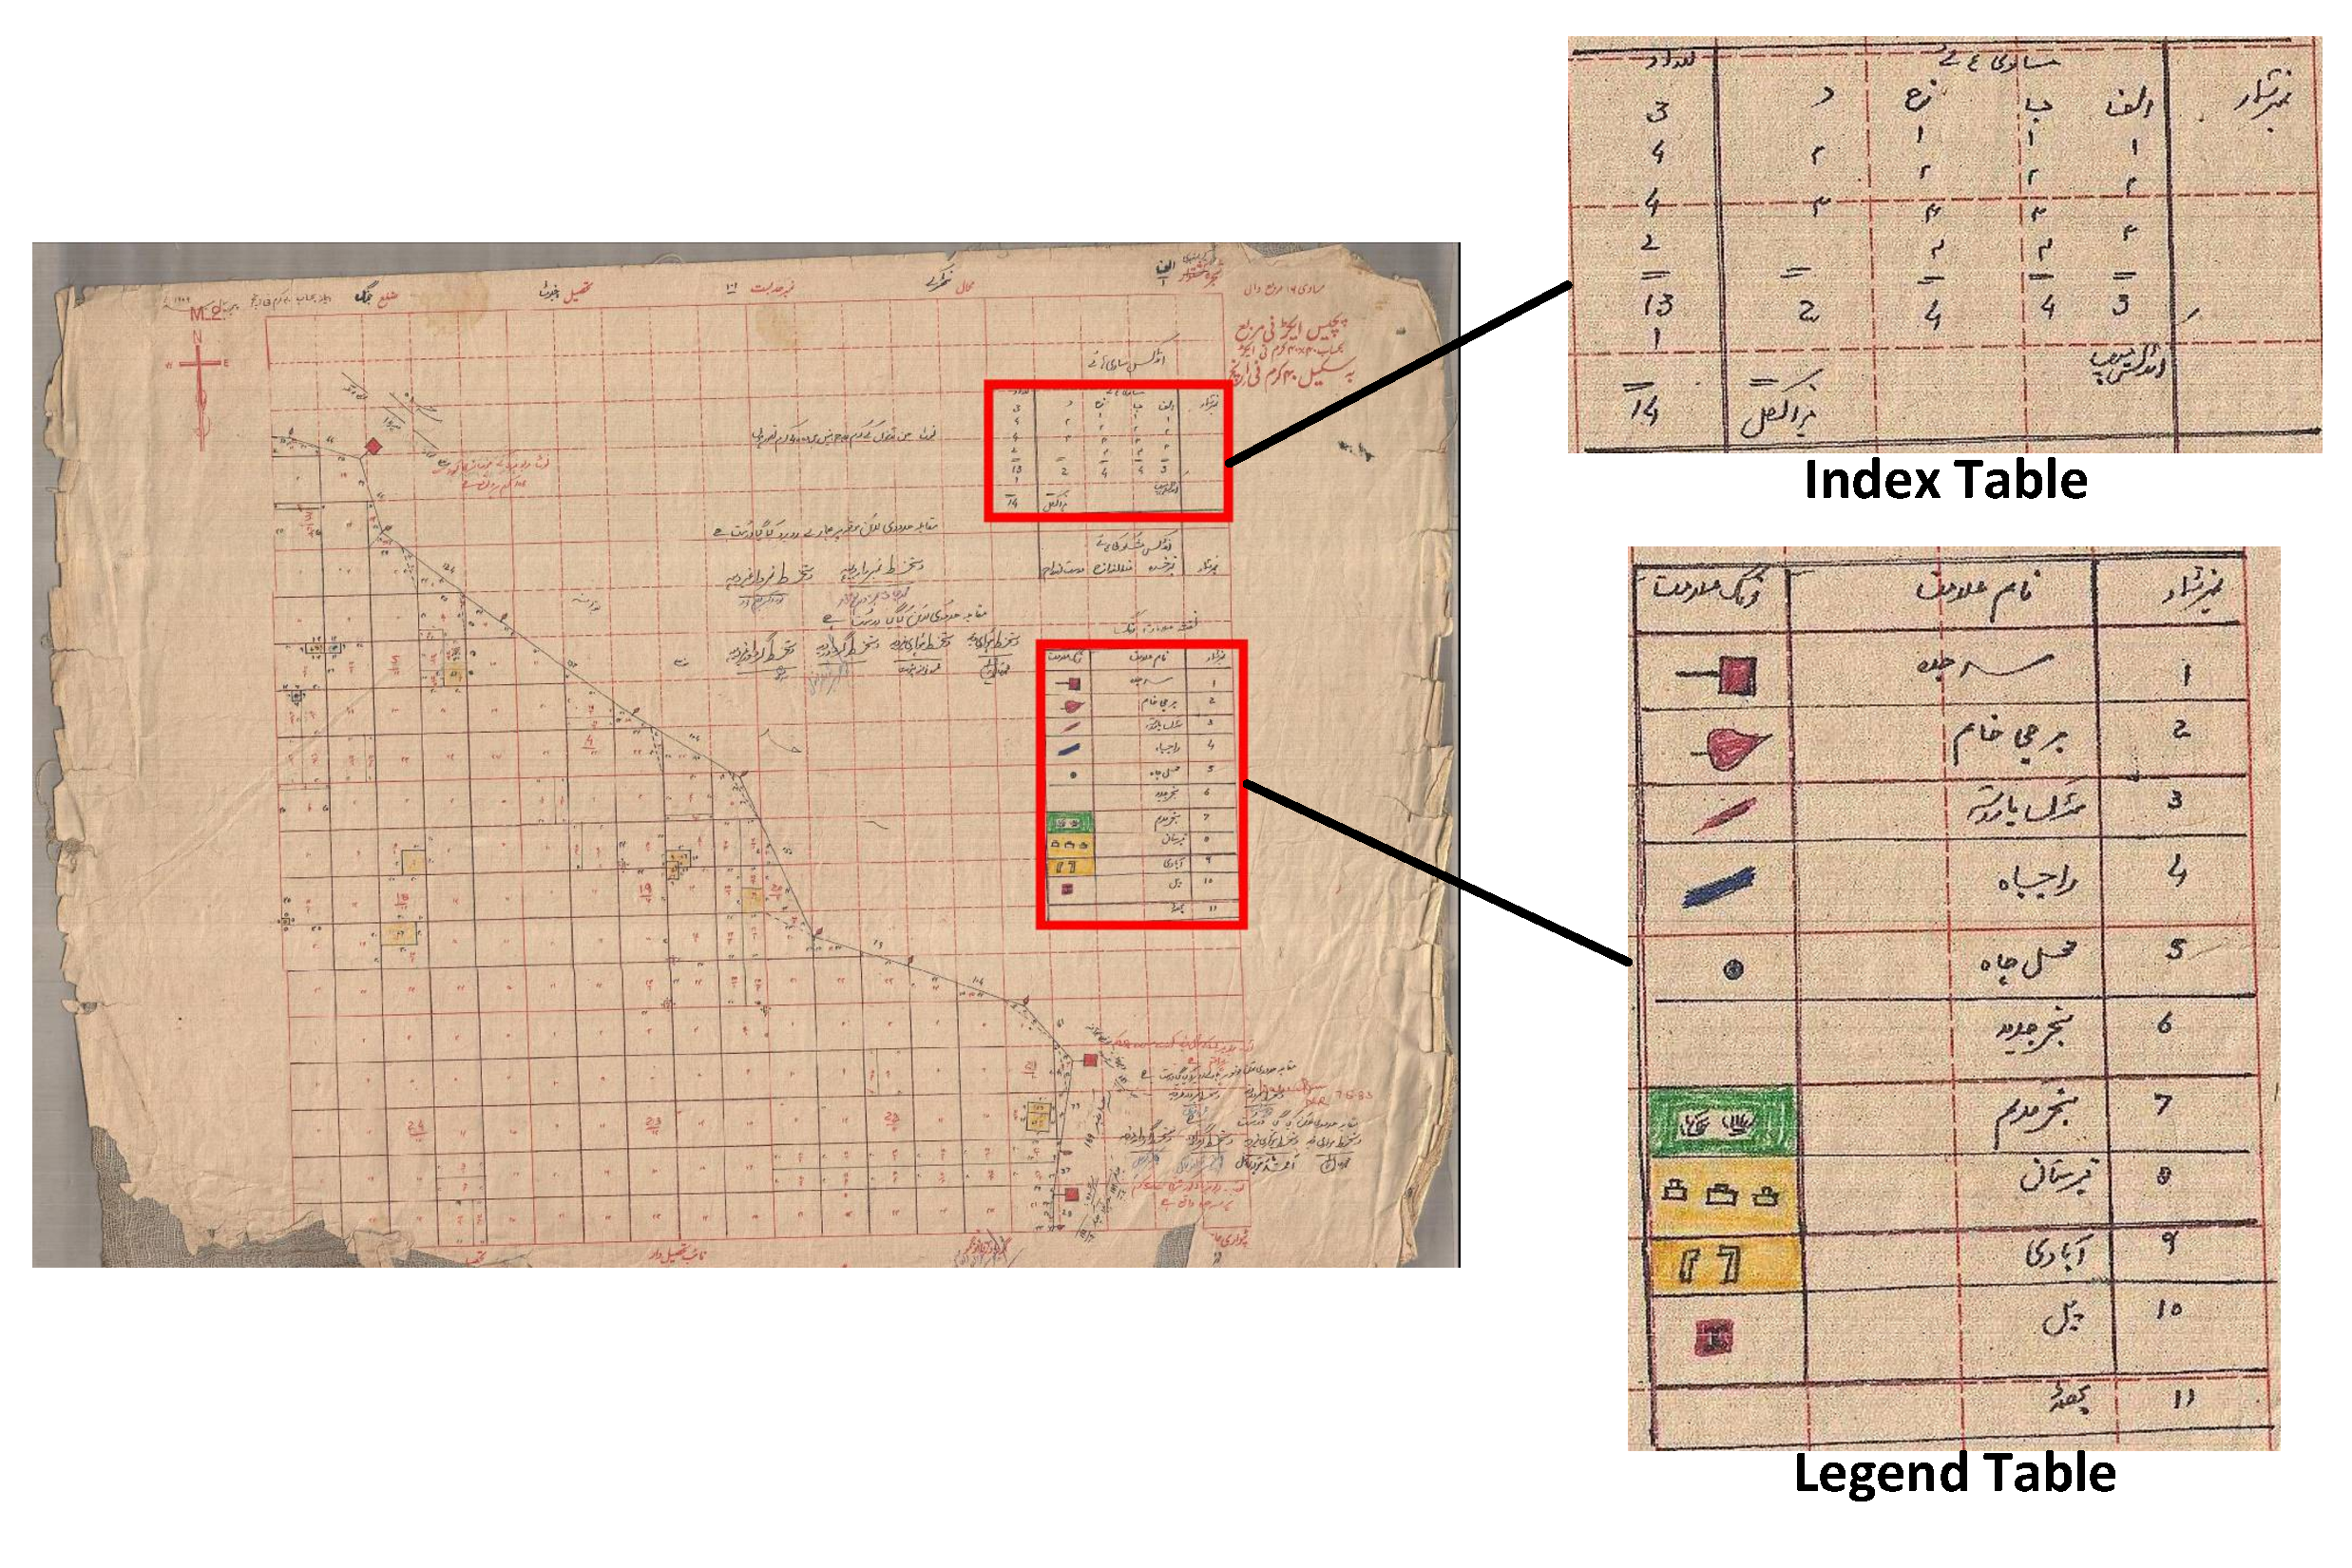
\includegraphics[width=\linewidth,keepaspectratio,angle=0]{Fig1_massavi_Tables.pdf}
    \caption{A map containing meta-data in the form%Left(masavi %image), right(Index and Legend Tables) from top to bottom %respectively.
    }
    \label{fig:masavi}
\end{figure}

Historical cadastral maps contain rich information useful for administrative decision making and longitudinal analysis. This can include information about land usage, numbers and sizes of land units, schools, hospitals and water resources. To capture any region on a fine resolution, multiple maps are required. For example, a village is usually represented via multiple constituent maps. For village-level digitization of information found in cadastral maps, the individual maps need to be digitized into a combined unit. To aid this process, maps often contain meta-information in the form of tables. \autoref{fig:masavi} shows a map that contains two types of tables:
\begin{enumerate}
\item an Index table that contains information about how the constituent maps are to be arranged together to form a village map (see \autoref{fig:IndividualMassavis_Mauza}), and
\item a Legend table that describes the different symbols on the maps (see \autoref{fig:legendTable}).
\end{enumerate}
\begin{figure}[h!]
    \centering
    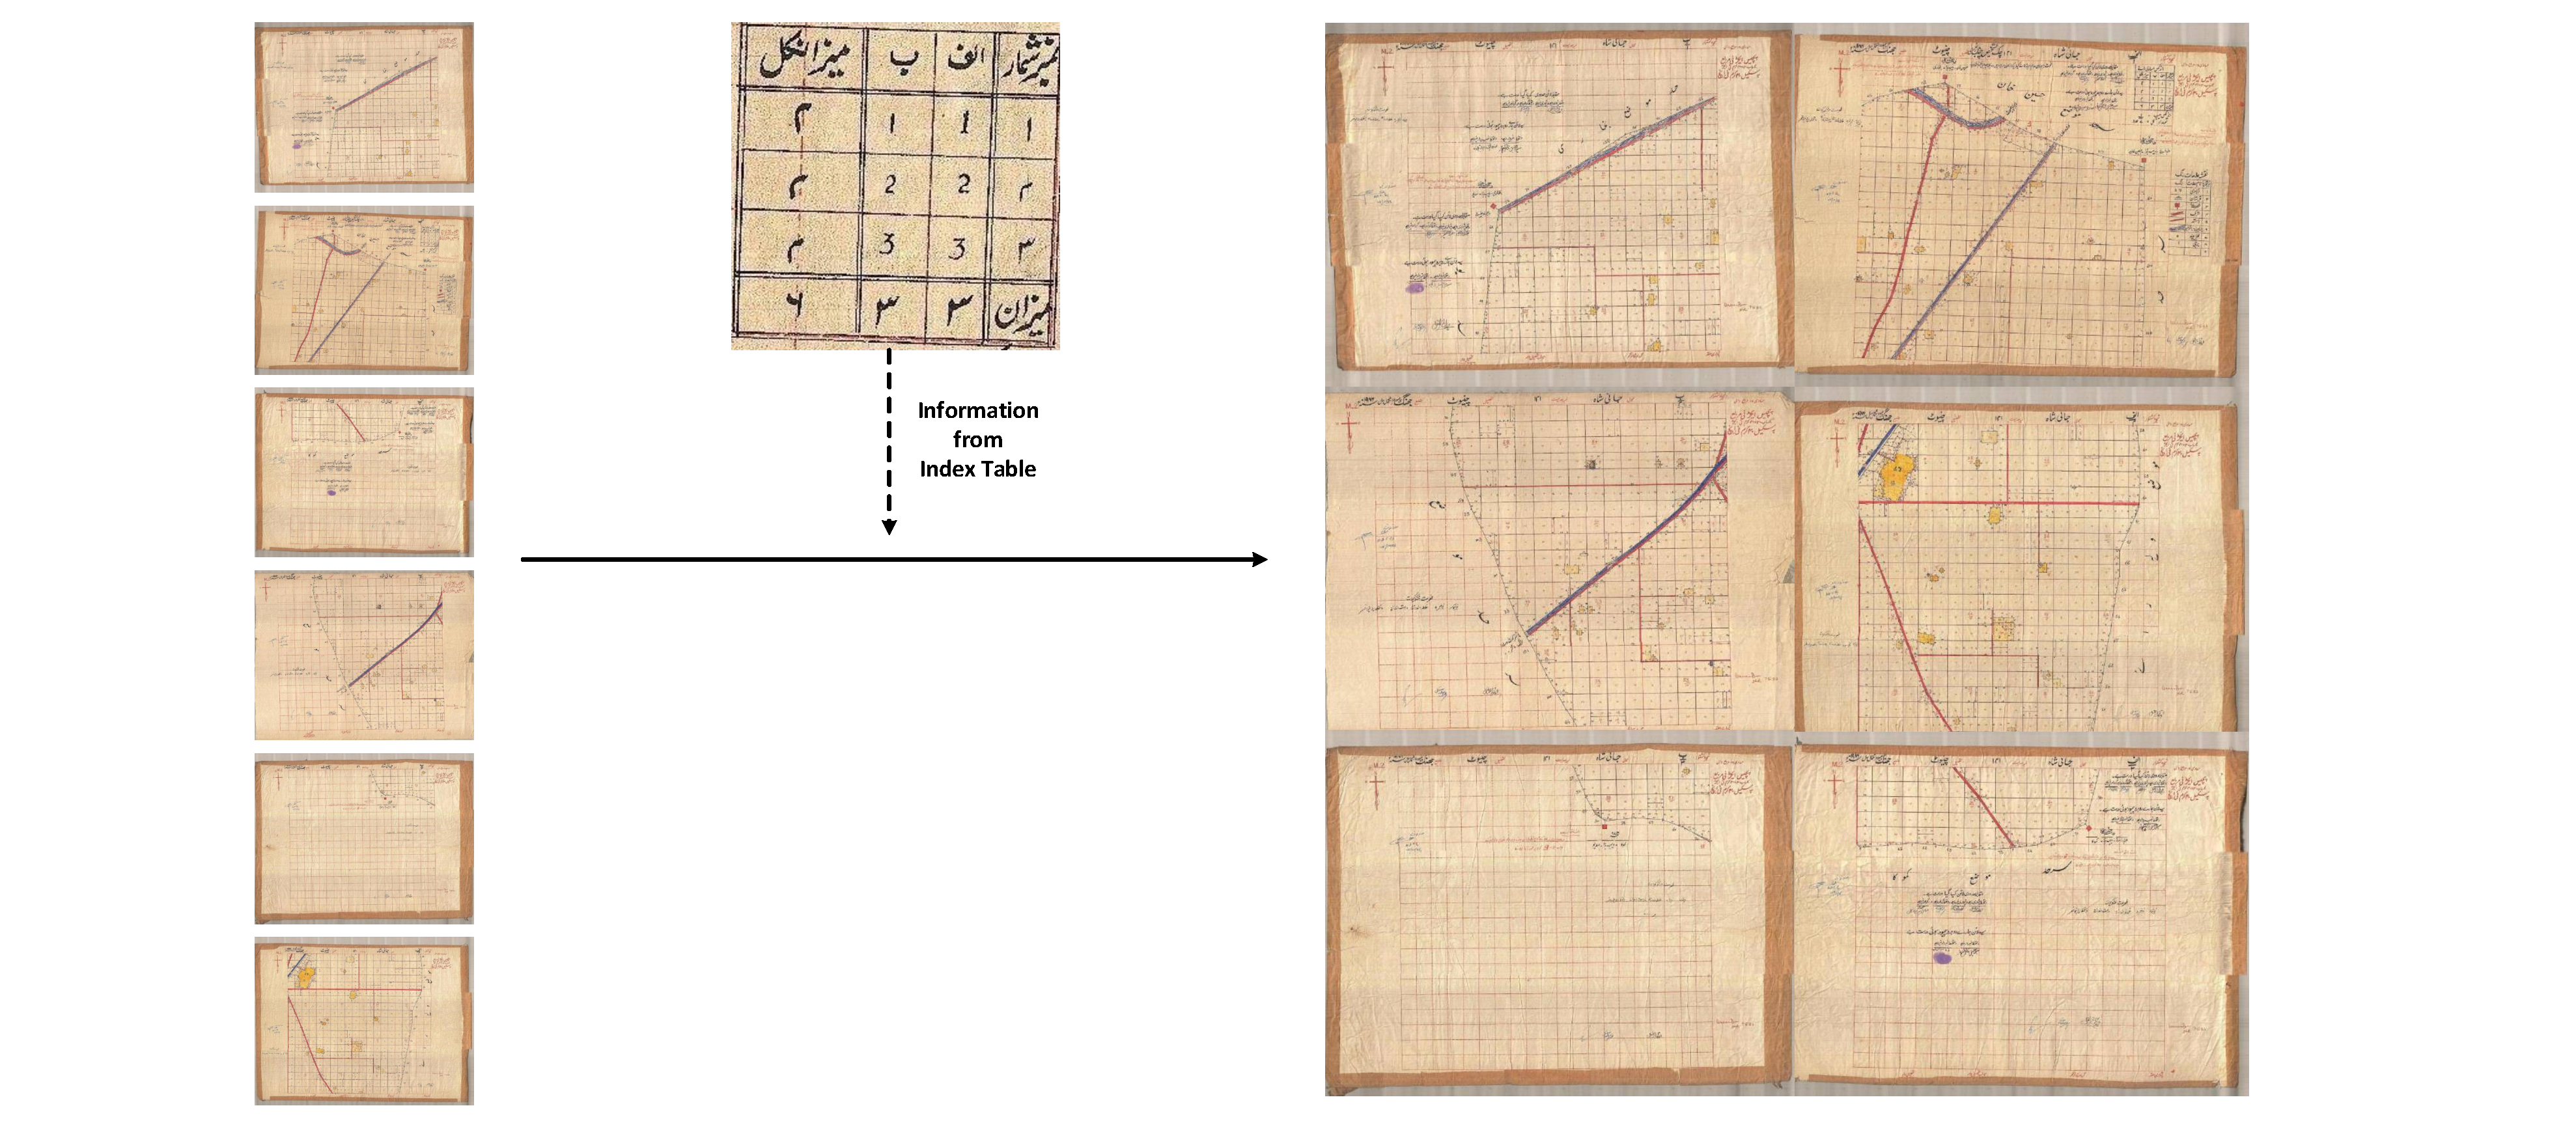
\includegraphics[width=\linewidth,keepaspectratio]{individualMassavis_IndexTable_Mauza.pdf}
    \caption{Constituent maps of village are shown at left side. These constituent maps can be combined using information contained in Index Table to form map of the whole village which is shown at the right side.}
    \label{fig:IndividualMassavis_Mauza}
\end{figure}
\begin{figure}[h!]
     \begin{center}
     \begin{tabular}{lll}
      \hline\noalign{\smallskip}
      \textbf{Symbol}& \textbf{Urdu Name} & \textbf{English Name} %& \textbf{Sr. No.} 
      \\ 
      \noalign{\smallskip}\hline\noalign{\smallskip}
      \raisebox{0in}{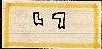
\includegraphics[width=0.25\linewidth,keepaspectratio]{abadi_symbol.jpg}}
      & 
      \raisebox{0in}{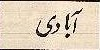
\includegraphics[width=0.25\linewidth, keepaspectratio]{abadi_name.jpg}}
      %& 
      %1
      &
      Settlement
      \\
      \raisebox{0in}{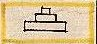
\includegraphics[width=0.25\linewidth,keepaspectratio]{qabristan_symbol.jpg}}
      & 
      \raisebox{0in}{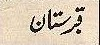
\includegraphics[width=0.25\linewidth, keepaspectratio]{qabristan_name.jpg}}
      %& 
      %2
      &
      Graveyard
      \\
      \raisebox{0in}{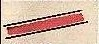
\includegraphics[width=0.25\linewidth,keepaspectratio]{sarak_symbol.jpg}}
      & 
      \raisebox{0in}{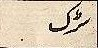
\includegraphics[width=0.25\linewidth, keepaspectratio]{sarak_name.jpg}}
      %& 
      %3
      &
      Road\\
      \noalign{\smallskip}\hline
      \end{tabular}
      \caption{Information contained in Legend Table.}
      \label{fig:legendTable}
      \end{center}
\end{figure}

Both kinds of information are usually recorded in the form of tables drawn on the map document. While tabular structure detection in printed documents has received attention over the years \cite{paliwal2019tablenet,qasim2019rethinking,khan2019table,kavasidis2019saliency,siddiqui2018decnt,arif2018table,schreiber2017deepdesrt,he2017multi,gilani2017table,shigarov2016configurable,kasar2015table,kasar2013learning,wang2004table,wangt2001automatic,kieninger1998t}, hand-drawn table detection has not been explored much \cite{ghanmi2014table,chen2012model,chen2011table}. More specifically, no prior work exists for table detection in historical cadastral maps where the problem involves additional challenges. For example, as \autoref{fig:masavi} shows, map documents are often drawn over a background grid that itself resembles a periodic, tabular structure. This makes  it harder to differentiate between a background grid and table drawn on top of it. This is in addition to historical document challenges such as wear and tear, ink leakage, and ink fading and hand-drawn document challenges such as uneven stroke width, missing strokes, inconsistent standards, non-orthogonal angles, not exactly straight lines, and text and graphics overlap.

In this work, we present a method for
\begin{enumerate}
      \item detection of tables in hand drawn cadastral maps,
      \item classification of the detected tables into Index and Legend tables,
      \item row and column detection in each table, and
      \item extraction of each cell of each table. 
\end{enumerate}
We have achieved $95.93\%$ $F_1$ score for table detection, $97.29\%$ $F_1$ score for row and column detection and $93.24\%$ $F_1$ score for cell detection.

Rest of the paper is organized as follows: Section II provides the related work for table detection and structure recognition. Section III describes the proposed methodology for detection, classification and structure recognition of index and legend tables. Section Iv is about dataset preparation and annotation. In section V experiments and results are discussed on all of the three tasks of detection classification and structure recognition. Section VI which is the last section of the paper concludes the paper.
\section{Related Work}
\label{sec:relatedWork}
Several attempts have been made on the topic of table detection and structure recognition. Traditional approaches mostly exploit heuristics, visual hints and formal table templates. We will mostly focus on methods utilizing deep learning techniques. 
\subsection{Table Detection}
\label{sec:relatedWork_Table}
Siddiqui et al. \cite{siddiqui2018decnt} proposed DeCNT to detect tables of arbitrary layout so as to cover wide range of diverse document images. DeCNT uses deformable convolution with state of the art Faster RCNN. Deformable convolution shapes its receptive field according to given input instead of simple convolution which has a fix receptive field. They show that by training their model on only ICADAR-2017 dataset, they achieved state of the art results on ICDAR-2013 test dataset. Results on Marmot and UNLV dataset are not compared with others but their model is performing very well also on these datasets which are not used for training. Arif et al. \cite{arif2018table} collected a large number of images from magazines, research articles, newspapers, annual reports, books and buisness letters to create a new dataset containing variety of tables. They annotated the data using labelImg tool. To capture foreground features they pre-processed the images b using coloration scheme. They have used red color to color code all the numeric data and green color for textual data. For capturing background features author applied distance transformation to color coded images. These pre-processed images are fed to Faster RCNN for training. For generalization test they evaluated their model on UNLV dataset. They compared their model's performance on UNLV dataset with Gilani at el. \cite{gilani2017table} reporting better results on their trained model. Their method builds on observation that there is more numeric data written in tables as compared to textual data. While in our dataset it is not the case. He et al. \cite{he2017multi} proposed multi scale and multi task FCN which semantically segments a document image into figures, text blocks and tables. FCNs are used to extract features of an image at multiple scale. For predicting the edges of each instance they exploited contour detection network. They used CRF conditional random fields to improve results from segmentation and contour detection network. They have performed experiments on real as well as synthetic data. To detect tables in handwritten documents Chen et al. \cite{chen2011table} separated text components of document image using SVM classifier, then measured coherence between adjacent text lines by employing correlation based approach. Gillani et al. \cite{gilani2017table} employed Faster RCNN for table detection task. They preprocessed the images before training and evaluated their model on publicly available UNLV dataset beating the Tesseract's table detection system by a reasonable margin.
\subsection{Table Structure Recognition}
\label{sec:relatedWork_Structure}
A considerable amount of work has been done to recognize structure of a table both using heuristic-based methods as well as deep learning methods. T-Recs was one of the earliest successful system for table structure recognition proposed by Kieninger et al. \cite{kieninger1998t}. The basic idea of T-Recs was not to use separators like lines and spacing rather they used a bottom-up approach which aggregates word segments into blocks making rows and columns based on horizontal and vertical overlaps. Their bottom up approach was based on intuition that human doesn't look at text lines and spacing rather he recognizes columns, rows or blocks as aggregation of words. Wang et al. \cite{wangt2001automatic} proposed an automatic ground truth generation system for table detection. table. Input to their table detection algorithm is line and word detection results which are modified according to column type of a given page. This preprocessed input is fed to coarse-to-fine table identification algorithm based on background analysis for detecting tabular regions. For table structure recognition they did vertical projections on all words which resulted in peaks and valley. They separated each column that starts from a valley and ends at the succeeding valley. Their table structure identification algorithm is similar to a recursive X-Y cut algorithm. After separating the columns they they identified cells and achieved 90\% correct detection of cells. Wang et al. \cite{wang2004table}proposed an optimization algorithm for table structure recognition. Their algorithm takes line segments and word entities as input and is based on probabilities which are estimated using geometric measurements from large training data. Their proposed algorithm works on single, double, and mixed column page layouts. Kasar et al. \cite{kasar2015table} proposed a table structure extraction system based on query-patterns. A client-driven approach is used in which the client provides a query pattern which is a set of key fields in image of document. Each key field is represented by a bounding box(x,y,h,w) and content which is a string. Query pattern is transformed to a relational graph and then a graph matching technique is used to extract similar graphs. After collecting all similar graphs, they analyzed these graphs to get column segments, row segments and then extracted the cells. Shigarov et al. \cite{shigarov2016configurable} proposed a method for structure recognition of tables in a PDF document which is untagged. They make use of heuristics such as ruling, horizontal distances, vertical distances, fonts and text chunks. Text chunks are grouped to make text blocks which are then used to extract rows columns and cells. Recently Khan et al. \cite{khan2019table} proposed a sequential model for structure recognition based on a fact that rows and columns in a table follow a sequential repetitive pattern of spacing and data length between next and previous rows and columns. Images of tables are first preprocessed for noise removal, binarization and transformation, then two bidirectional GRUs are used, one bidirectional GRU for identifying row boundaries and the other for identifying column boundaries. Each bidirectional GRU is followed by a fully connected layer for classifying input as either a row boundary or a column boundary. They have benchmarked their system on publicly available UNLV dataset which they didn't used in training process. Moreover they compared the performance of two different architectures of RNN, GRU and LSTM on both row and column classification and analyzed that GRU is beating the LSTM by a significant margin for both tasks.
\subsection{Table Detection and Structure Recognition}
\label{sec:relatedWork_Table_Structure}
Paliwal et al. \cite{paliwal2019tablenet} proposed end to end deep learning model for table detection and structure recognition by VGG-19 pretrained on ImageNet dataset as its base network followed by two branches, one for tabular region detection and the other for segmentation of columns within that tabular region. Also pixel wise predictions are made for detecting tabular regions as well as column region to avoid noise. For pixel wise prediction which is known as semantic segmentation they exploited FCN architecture provided by Long et al. \cite{long2015fully} which uses encoder-decoder network architecture, features extracted from encoder are shared by two decoders, one decoder outputs tabular region and other outputs column regions. For extracting rows they did not use a third decoder but used rule-based row extraction method so as to extract data from each cell of the table by using rows and columns. Row extraction is done by using heuristics such as lines separating each row, blank spaces, word patches which are at the same level are considered as one row. While in our method we have not used any heuristics to extract rows as well as column and tabular regions.  They have shown result for table detection and column detection but they didn’t show result for row extraction. In our thesis we will show result for row extraction as well. In addition we have also classified the tables into their types on the basis of their content, not reading the header of the table which contain name of the table because in our dataset not all the tables have names in their headers. They evaluated their technique on publicly available ICDAR and Marmot datasets. They provided annotations of Marmot dataset for structure recognition which were not been available before. To the best of my knowledge, Schreiber et al. \cite{schreiber2017deepdesrt} are the first who adapted domain of object detectors to detect tables in document images. Their method is applicable to images rather than PDFs which can be easily converted to images. They have used two emerging concepts of transfer learning and domain adaptation for both detection and structure recognition of tables. They considered table detection and structure recognition as two separate problems. A deep learning based solution is proposed in their paper which utilizes Faster R-CNN for table detection. For structure recognition, first they produced results using the same Faster R-CNN. To improve the performance on very closely spaced rows, they exploited FCN-2s architecture by exchanging scale layers for normalization layers. They achieved state of the art results on publicly availble ICDAR and Marmot datasets. We are also doing classification of table type and we are using semantic segmentation to predict pixel wise mask for predicting rows and columns. Qasim et al. \cite{qasim2019rethinking} contended that Graph Neural Network are more suited for table recognition problem instead of standard Neural Networks. They open sourced their code for generating large amount of synthetic data which was main hurdle for using deep learning approaches. Also they opened source their implementation of training graph neural network to let researchers work in this direction. They covered different categories of Tables based on difficulty such as table with borders and plain rows and columns, Table without borders and separating lines of column and rows, Table with nested columns, table rotated at small angle having nested rows. They defined their problem using graph theory, ground truth for each table are three graphs. True positive rate, False positive rate and perfect matching are their evaluation measures. Li et al. \cite{li2019tablebank} provided TableBank dataset which consists of 417K labelled images for table detection and structure recognition. According to author's view, datasets already available for table detection were very small, fine tuning pretrained networks on these small datasets have not good generalization capability on real world images. Author exploited the information inside the source code of word and latex documents to label the data. To demonstrate the effectiveness of TableNet on table detection task, they used Faster RCNN. while for structure recognition they trained image-to-text model provided by OpenNMT which is an open source framework. Although TableNet provides good generalization but it is good for electronic documents. Kasar et al. \cite{kasar2013learning} proposed a method which uses horizontal lines, vertical lines and their intersection points to detect tables in document images by using a learned SVM classifier. Their method doesn't use any textual information inside the table which makes it good for locating tables containing any kind of textual information. Also the proposed method is unaffected by page layout but it totally depends on presence of ruling lines in tables which limits its use. We are working on a dataset which contains mixture of tables with or without borders and rulings lines. Also in our dataset of historical cadastral maps there are background grid line as well. Clinchant et al. \cite{clinchant2018comparing} compared two machine learning methods (Graph Convolutional Network and  Conditional Random Fields) and evaluated the performance of both approaches on historical register book containing hand written death records. Their main problem was row extraction because of handwriting and style of different writers, some place more space between rows, some have thin writing and place less space between rows. After identifying columns and text lines they used BIESO categorization to build the rows ultimately reaching the cells using column and row information. Anand Gupta et al. \cite{gupta2019table} proposed a technique for table detection which is independent of ruling lines. To remove dependency of ruling lines they preprocess image to remove horizontal and vertical lines, this preprocessed image is then sent to a Tesseract engine which gives bounding box coordinates for all word blobs, these word blobs are then grouped into text lines based on horizontal threshold. Table region is then detected by finding minimum upper left coordinate and maximum bottom right coordinate for all word blobs. This technique uses number of hyper-parameters for computing rows and columns. Authors reported in their paper that their method is susceptible to errors when  document images contain grid plots, graphs or line diagrams. While we detect tables from cadastral maps which are drawn on background grid plots and contains graphical symbols as well. Devashish Prasad et al. \cite{prasad2020cascadetabnet} proposed an end to end method for predicting table and cell masks detection utilizing Cascade Mask R-CNN HRNet model for both tasks. There are two separate branches for predicting bordered and borderless tables in the proposed approach. Detection of table and cell masks at the same time may yield cell masks even when table is not detected. Chen et al. \cite{chen2012model} proposed a method based on location of key points for simultaneous detection and structure recognition of tables in noisy handwritten documents. They detected key points using graph cut algorithms. Ghanmi et al. \cite{ghanmi2014table} used Conditional Random Field approach for labeling each line in a line-segmented document image as TableRow or LineText. TableRow label is used for a line which belongs to a table while LineText label is used for a line which belongs to a text block. They reported that 88\% of table lines are detected correctly. Their approach is based on line-segmented document while the dataset we are working can not be segmented into lines. In our dataset there are images of maps in which text is not written in a line manner.

\section{Proposed Methodology}
\label{proposedMethodolgy}
The workflow of our proposed method is shown in \autoref{fig:workflow}. First, we detect all tabular instances in the input image. Each instance is also classified into a table category. Then each table is decomposed  into  rows  and  columns  which  are  finally  intersected to extract cells.
%This section gives detail about the proposed system for detection and structure recognition of Index and Legend tables in map documents. It consists of two separate parts. In the first part we will detect and classify tables in map images. Here detection is locating tables in masavis and classification is classifying the detected tables as Index or Legend. In the second part we recognize the structure (rows, columns and cells) of Index and Legend tables. 
%A brief overview of workflow we have followed to solve our problem is given in \autoref{fig:workflow}.

\begin{figure}[h!]
\centering
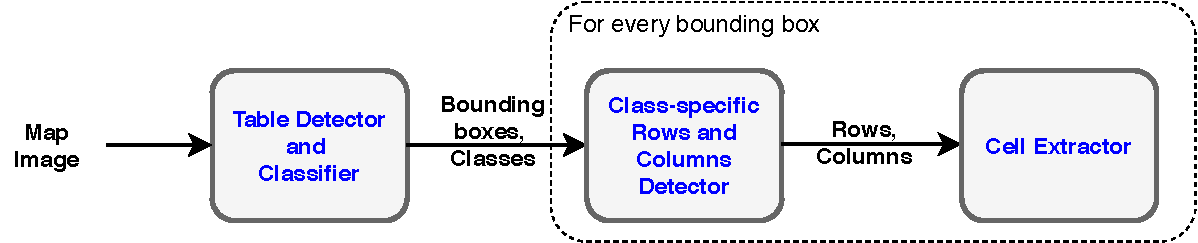
\includegraphics[width=\linewidth,keepaspectratio,angle=0]{workflow_small.pdf}
\caption{Proposed cell extraction pipeline. First, all tabular instances are detected. Then each table is decomposed into rows and columns which are finally intersected to extract cells.} %Workflow of proposed methodology at testing time. A massavi image is given as input to table detection and classification model, which outputs table bounding boxes and class (index or legend) for each table. Detected Index Table is then given as input to row and column detection (RCD) model which is trained on both Index and Legend Table, this model outputs row and column bounding boxes, mask and class (row or col) for Index Table. Detected Legend Table is given as input to row and column detection model pretrained on both Index and Legend Tables and specifically trained on Legend Tables, this model outputs row and column bounding boxes, mask and class (row or col) for Legend Table. A cell computation algorithm then computes cell bounding boxes for Index and Legend Tables by taking detected rows and columns an input.  }
\label{fig:workflow}
\end{figure}

\subsection{Detection and Classification of Tables in Masavis}
\label{sec:methodology_Table}

\begin{table*}
\caption{Resnet-101}
\label{tbl:resnet-101}
\centering

\small
\setlength{\tabcolsep}{0pt}
\begin{tabular*}{\textwidth}{@{\extracolsep{\fill}}lcccc@{}}
\hline\noalign{\smallskip}
conv 1 & conv 2 & conv 3 & conv 4 & conv 5\\
\noalign{\smallskip}\hline\noalign{\smallskip}
\bsplitcell{7\texttimes7 conv, 64, stride=2\\
3\texttimes3 max pool, stride=2} 
&
  \bsplitcell{1\texttimes1 , 64  \\ 3\texttimes3 , 64 \\ 1\texttimes1 , 256}\texttimes3 &
  \bsplitcell{1\texttimes1 , 128  \\ 3\texttimes3 , 128 \\ 1\texttimes1 , 512}\texttimes4
  &
  \bsplitcell{1\texttimes1 , 256  \\ 3\texttimes3 , 256 \\ 1\texttimes1 , 1024}\texttimes23
  &
  \bsplitcell{1\texttimes1 , 512  \\ 3\texttimes3 , 512 \\ 1\texttimes1 , 2048}\texttimes3
\\
\noalign{\smallskip}\hline
\end{tabular*}
\end{table*}

\begin{figure*}[h!]
\centering
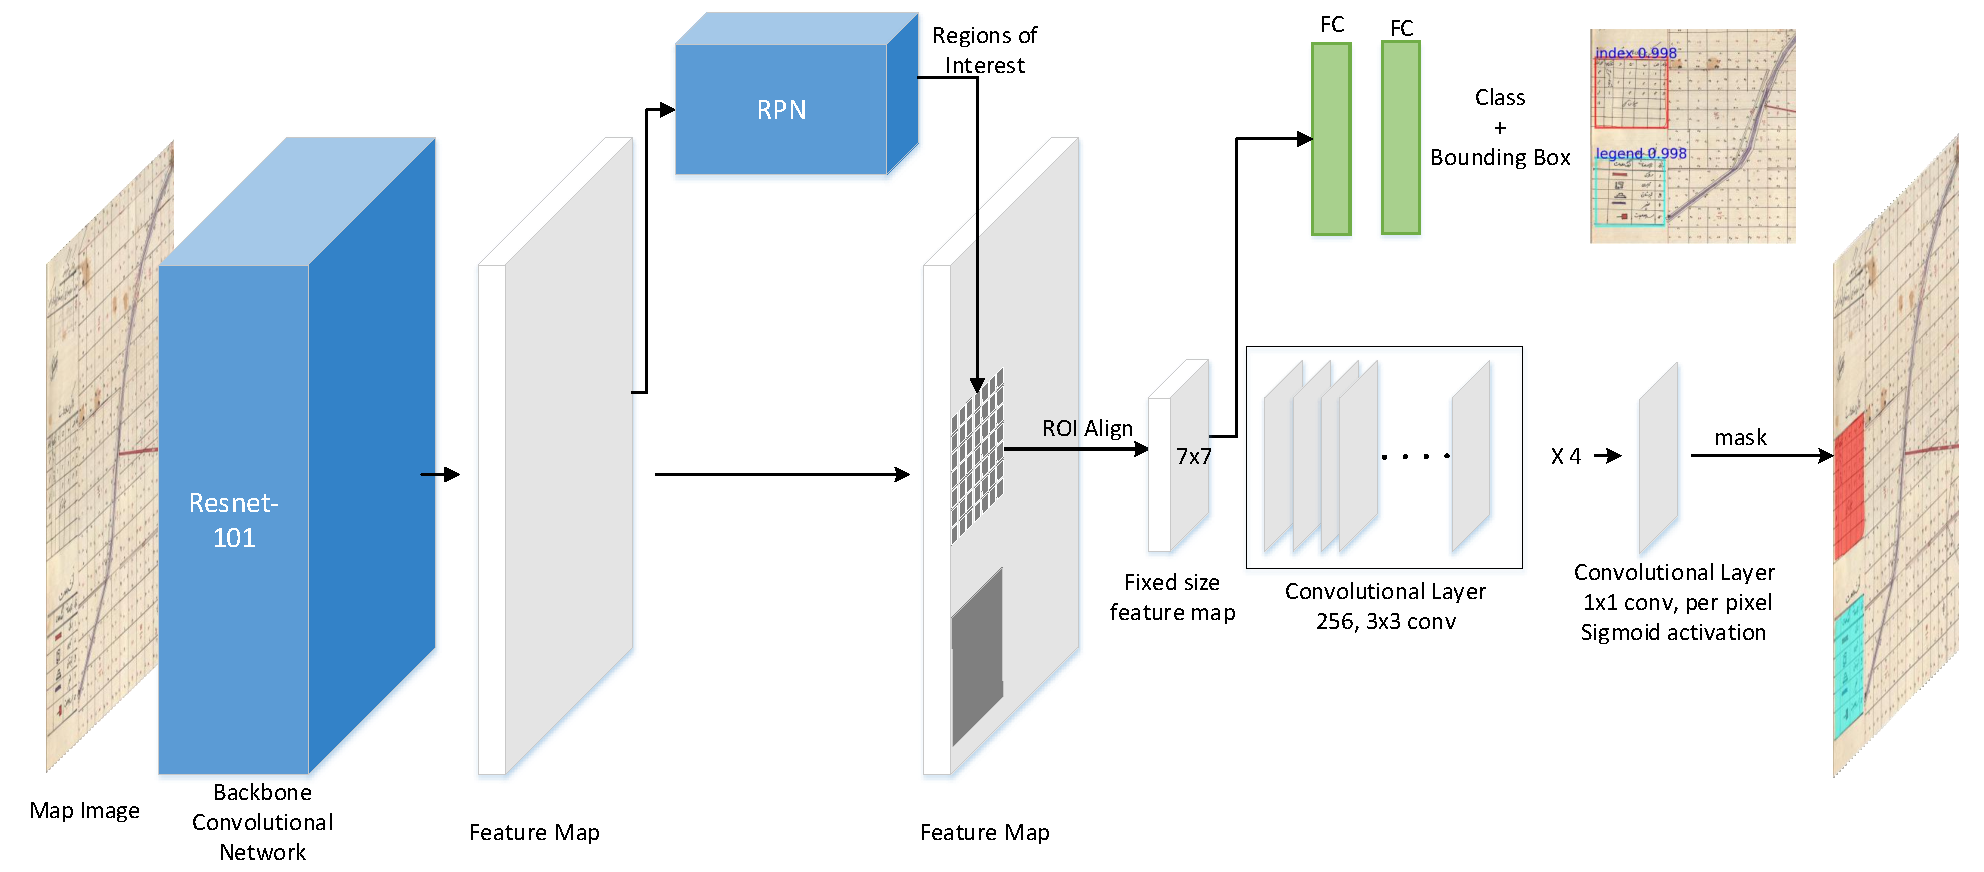
\includegraphics[width=\linewidth, angle=0,keepaspectratio]{method_mask_rcnn.pdf}
\caption{Table detection using Mask R-CNN. FC is a fully connected layer, RPN is region proposal network, ROI is region of interest. For better visibility of diagram zoom the document.}
\label{fig:maskRCNN_table}
\end{figure*}

We treat tables as objects. Object detection and classification has seen rapid progress over the last decade [\memonazar{ASMAT, PLEASE CITE SOME OF THE MAIN OBJECT DETECTORS}\memoasmat{ Done.} \cite{girshick2014rich,girshick2015fast,ren2015faster,redmon2016you,liu2016ssd,dai2017deformable,he2017mask,zhang2018single}]. By considering tables as objects, we leverage the potential of existing object detection frameworks. Just like natural objects, tables can be visually distinguished from other background content due to their particular structure. So existing object detection models should be able to detect tables as well. Our results verify this hypothesis.

%To detect Index and Legend Tables in a masavi image our idea was to treat these tables as objects and use the potential of existing object detection frameworks. Just like natural objects, tables can be visually distinguished from other background content due to their particular structure. So existing object detection models should be able to  perform well with the problem of table detection as well. Our results verify this hypothesis.

We choose the Mask R-CNN model \cite{he2017mask}. It is a deep object detection model with two stages. In the first stage, a region proposal network (RPN) proposes regions of interest. In the second stage, it predicts bounding box estimates and region masks of tabular instances along with their classification labels. We do not make use of the region masks in this work. %it predicts bounding box offsets which are regressed by a bounding box regressor, class and a binary mask for each region of interest. For table detection we don't care about mask. Both stages share features from a backbone Resnet-101 convolutional network. Mask R-CNN architecture for table detection is shown in \autoref{fig:maskRCNN_table}.

\begin{figure*}[h!]
\centering
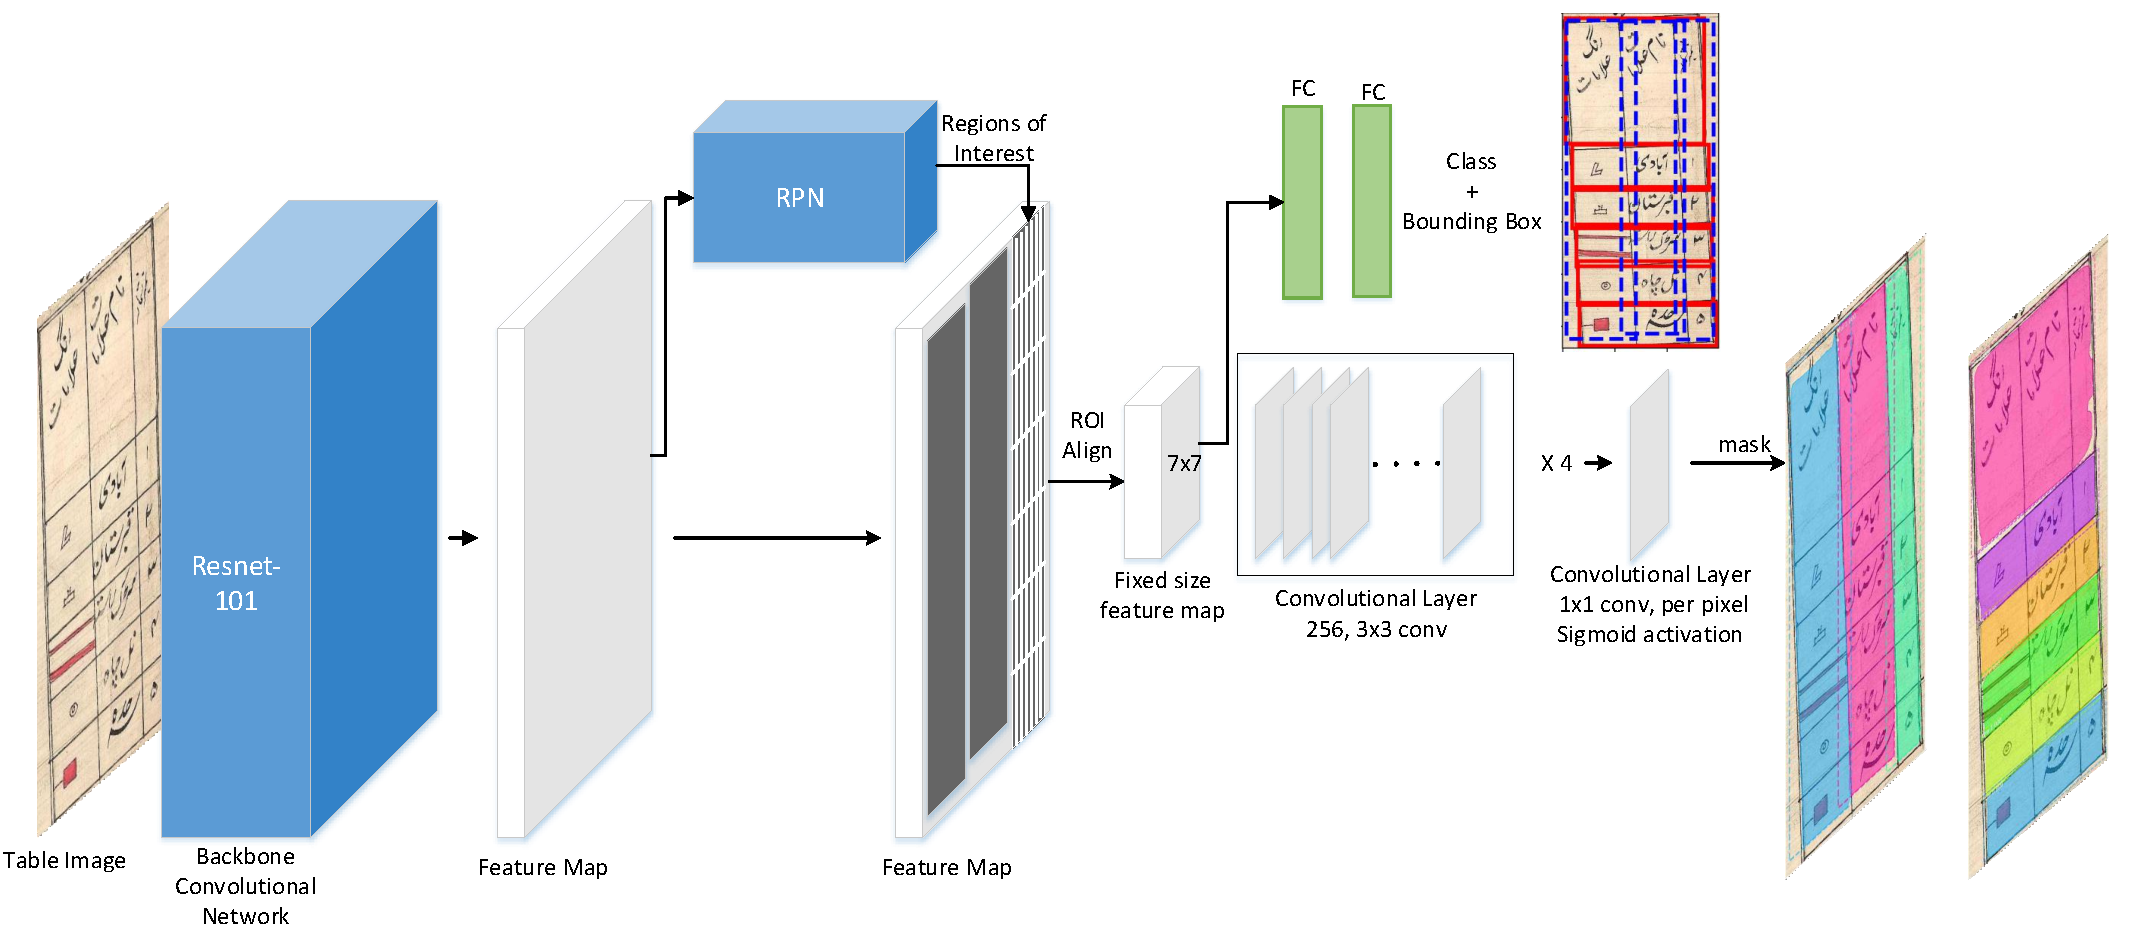
\includegraphics[width=\linewidth, angle=0,keepaspectratio]{methodrow_col_mask_rcnn.pdf}
\caption{Row and Column detection using Mask R-CNN. FC is a fully connected layer, RPN is region proposal network, ROI is region of interest. For better visibility of diagram zoom the document}
\label{fig:maskRCNN_row_col}
\end{figure*}
Features maps of input image are extracted using Resnet-101 convolutional network. Resnet-101 consists of 5 stages. In the first stage, input image is 3 pixel padded with zeroes from all sides. This zero padded input image is then passed to a convolutional layer with 64 feature maps, each feature map with 7x7 convolutional filter with stride of 2. Convolutional layer is followed by a MaxPooling layer. Size of output of MaxPooling layer is same as size of input which is achieved using padding. Detailed architecture of convolutional layers in Resnet-101 excluding last fully connected layer is given in \autoref{tbl:resnet-101}. Feature map from last convolutional layer of Resnet-101 is fed into RPN, a region proposal network which gives rectangular region of interests, each region of interest with an objectness score. RPN proposes regions by sliding a small network over the input feature map. This network is fully connected with 3x3 spatial window of feature map which is mapped to 256 dimensional vector followed by two sibling layers, one with linear activation function for predicting bounding box for proposed region and other with softmax activation function for classifying the proposed region as containing an object or not. Each proposed region on feature map is mapped to a fixed feature map (7x7) using ROI Align instead of ROI pool which comes up with misalignment issue while making quantization and pooling. For predicting pixel wise mask for segmenting instances we need to fix this misalignment issue. Mask R-CNN proposed ROI Align Layer to avoid this pixel-to-pixel misalignment between region of interest and small fixed size feature map by using bilinear interpolation. This fixed size feature map (7x7) is fed into fully connected layers followed by another fully connected layer which is followed by two sibling layers for predicting class and bounding box for the proposed region. For mask prediction, fixed size feature map is fed into convolutional layers with relu activation function followed by 1x1 convolution with per pixel sigmoid activation function to predict binary mask. 
\subsection{Table Structure Recognition}
\label{sec:methodology_structure}
\subsubsection{Row and Column Detection}
\label{sec:methodology_structure_rowCol}
The same idea for table detection can be applied to detect rows and columns. The important thing to note here is that bounding boxes for rows and columns can overlap because we are working on hand-drawn maps and there is no standard method used here to draw tables, there are sloped lines for row and column boundaries.
The whole table is sloped to a small degree. So,we need bounding box as well as instance segmentation mask for each row and  column.
Mask R-CNN segments the objects giving a mask for each object. So, we have trained Mask R-CNN model for detection and instance segmentation of rows and columns. Given an image of table, Mask R-CNN detects rows and columns in the table giving (i) bounding boxes for rows and columns (ii) class for each bounding box (iii)segmentation mask for each row and column. Proposed methodology for row and column detection is shown in \autoref{fig:maskRCNN_row_col}.
\subsubsection{Cell Computation}
\label{sec:methodology_structure_cell}
To reach the cells of table we used rows and columns which are detected from row column detection model. In our cell computation algorithm, we first sort all detected rows and all detected columns. Then we compute overlap of all rows and all columns to get each individual cell with its bounding box coordinates and its position (row no. , column no.) in table.
\section{Dataset Preparation}
\label{datasetPrep}
We have 2339 scanned images of masavis for digitization of cadastral maps which were collected by our colleague also working on this project. All of these 2339 images of masavis do not contain index and legend tables. For detection and recognition of index and legend tables we separated those masavi images which contain index or legend table or both and made a smaller dataset which we named as \textbf{MapIndexLegendTables}. MapIndexLegendTables dataset consists of 356 images of masavis which contain index and legend tables.\newline
For row and column detection we cropped all index and legend tables from all of the 356 masavi images in MapIndexLegendTables and saved them as images and named this dataset of tables as \textbf{MapTablesRowCol}. MapTablesRowCol dataset contains 616 images of index and legend tables.
\begin{table}[h!]
\caption{Dataset Split for Table Detection}
\label{tbl:trainTestImgCount_tableDet}
\centering
\resizebox{\linewidth}{!}{%
\begin{tabular}{| c | c | c |c |}
\hline
\multicolumn{4}{|c|}{\textbf{Total Map Images}=356}\\
\hline
\multicolumn{2}{|c|}{\textbf{Training Images}=284} &\multicolumn{2}{|c|}{\textbf{Testing Images}=72}\\
\hline
 \textbf{Index Tables} & \textbf{Legend Tables}  &\textbf{Index Tables} & \textbf{Legend Tables}  \\ 
 \hline
  228 & 269 & 51 & 72 \\
  \hline
\end{tabular}
}
\end{table}
\begin{table*}[h!]
\caption{Dataset Split for Row and Column Detection}
\label{tbl:trainTestImgCount_rowColDet}
\centering
\resizebox{\textwidth}{!}{%
\begin{tabular}{| c | c | c |c | c |c | c | c | c |c | c |c |}
\hline
\multicolumn{12}{|c|}{\textbf{Total Table Images}=616}\\
\hline
\multicolumn{4}{|c|}{\textbf{Training Images}=495}&\multicolumn{4}{|c|}{\textbf{Validation Images}=60} &\multicolumn{4}{|c|}{\textbf{Testing Images}=61}\\
\hline
 \multicolumn{2}{|c|}{\textbf{Index Tables}=226}& \multicolumn{2}{|c|}{\textbf{Legend Tables}=269}  &\multicolumn{2}{|c|}{\textbf{Index Tables}=25} & \multicolumn{2}{|c|}{\textbf{Legend Tables}=35}&\multicolumn{2}{|c|}{\textbf{Index Tables}=25} & \multicolumn{2}{|c|}{\textbf{Legend Tables}=36}\\
  \hline
   Rows & Columns & Rows & Columns & Rows & Columns & Rows & Columns & Rows & Columns & Rows & Columns  \\
  \hline
  1271 & 1139 & 2327 & 811 & 156 & 130 & 293 & 105 & 133 & 123 & 298 & 109  \\
  \hline
\end{tabular}
}
\end{table*}
\subsection{Dataset Annotation for Detection and Recognition of Index and Legend Tables}
\label{sec:dataset_table}
For marking ground truths we used \textbf{labelimg} tool in which we open an image of masavi and draw a rectangle over each table saving the ground truth coordinates and class of each table in an XML file. coordinates are the four integer values one pair($x_1,y_1$) for top-left corner and one pair($x_2,y_2$) for bottom-right corner of rectangle containing table object. Class label is index for index table and legend for legend table. We did this for all of the 356 images in MapIndexLegendTables. So we created 356 XML annotation files. One XML file against one masavi image.
\begin{figure}[h!]
    \centering
    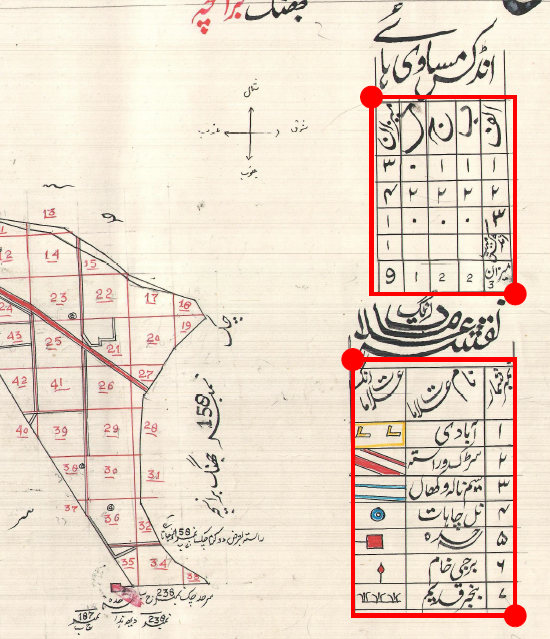
\includegraphics[width=\linewidth,height=5cm,keepaspectratio]{annot_massavi_tables.png}
    \caption{Annotation for detection of index and legend tables.}
    \label{fig:TableAnnot}
\end{figure}
\subsection{Dataset Annotation for Row and Column Detection}
\label{sec:dataset_rowCol}
Using \textbf{labelme} tool we marked ground truth coordinates( top-left corner and bottom-right corner), class and mask for each row and column of a table in MapTablesRowCol dataset. On average there are 56 clicks for marking ground truth coordinates of row and columns of one table. We did this for all of the 616 tables in MapTablesRowCol dataset. Class label for row is row and column is col. Ground truths for each table are saved in separate JSON files. For 616 images of table we have 616 JSON annotation files.
\begin{figure}[h!]
\centering
\begin{subfigure}{0.47\linewidth}
  \centering
  % include first image
  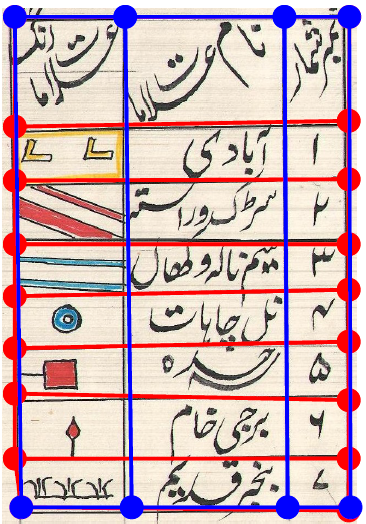
\includegraphics[width=\linewidth,height=5cm,keepaspectratio]{annot_legend_row_col.png}
    \caption{Legend Table}
    \label{Annotation for legend table}
\end{subfigure}
\begin{subfigure}{0.47\linewidth}
  \centering
  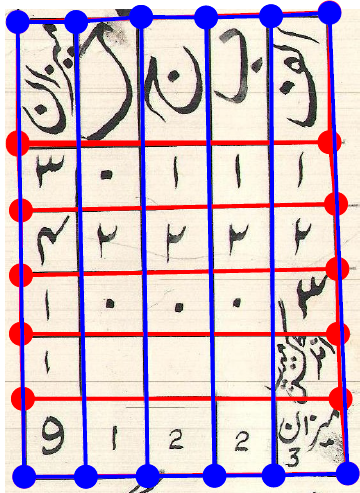
\includegraphics[width=\linewidth,height=5cm,keepaspectratio]{annot_index_row_col.png}
    \caption{Index Table}
    \label{Annotation for index table}
\end{subfigure}
\caption{Annotation for structure recognition of index and legend table.}
\label{fig:annot_rowcol}
\end{figure}
\section{Experiments and Results}
\label{expResults}
In this section we will show visual as well as numerical results. We will also give details of how we setup the environment and trained our model. The presented approach is evaluated on MapIndexLegendTables and MapTablesRowCol datasets which are introduced in section IV. We run all the experiments on GPU system having 16GB RAM with CUDA 8.0.61 installation and cuDNN 8.0 deep neural network library.
This section consists of three parts. In the first part we will provide detail of experiments and results for detection and classification of Index and Legend Tables. Second part shows results for structure recognition of Index and Legend Tables. Third and the last part shows results for cell detection.
\subsection{Detection and Classification of Index and Legend Table}
\label{sec:expResults_table}
\begin{table*}[h!]
\caption{Results for Table Detection}
\label{tbl:table_detection}
\centering
\resizebox{\textwidth}{!}{%
\begin{tabular}{| c | c | c |c | c | c |c | c | c |c | }
\hline
&\multicolumn{3}{|c|}{\textbf{IoU=0.5}} &\multicolumn{3}{c|}{\textbf{IoU=0.75}}& \multicolumn{3}{c|}{\textbf{IoU=0.9}}\\
\hline
 &\textbf{P@0.5} & \textbf{R@0.5}  & \textbf{$F_1$@0.5} & \textbf{P@0.75} & \textbf{R@0.75}  & \textbf{$F_1$@0.75}& \textbf{P@0.9} & \textbf{R@0.9}  & \textbf{$F_1$@0.9} \\ 
 \hline
 \textbf{Table (Index and Legend)} & 95.93\% & 95.93\% & 95.93\% & 91.87\% & 91.87\% & 91.87\% & 75.61\% & 75.61\% & 75.61\% \\
 \hline
 \textbf{Index Table} & 92.16\% & 92.16\% & 92.16\% & 82.24\% & 82.24\% & 82.24\% & 72.55\% & 72.55\% & 72.55\%\\
 \hline
 \textbf{Legend Table} & 97.22\% & 97.22\% & 97.22\% & 93.06\% & 93.06\% & 93.06\% & 76.39\% & 76.39\% & 76.39\%\\
 \hline
\end{tabular}
}
\end{table*}

\begin{figure*}[h!]
\centering
\begin{subfigure}{0.325\linewidth}
  \centering
  % include first image
  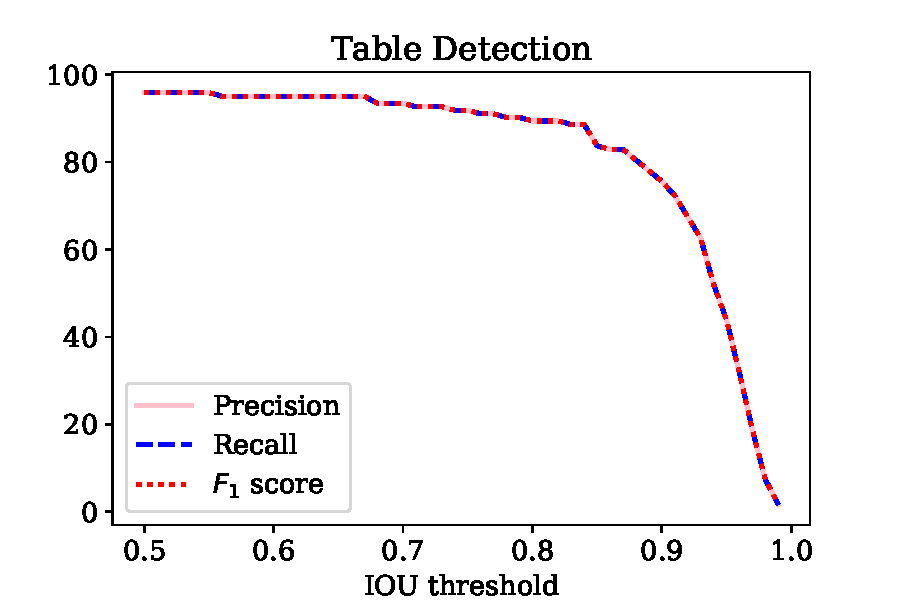
\includegraphics[width=\linewidth]{table_pRf.pdf}
    \caption{}
    \label{}
\end{subfigure}
\begin{subfigure}{0.325\linewidth}
  \centering
  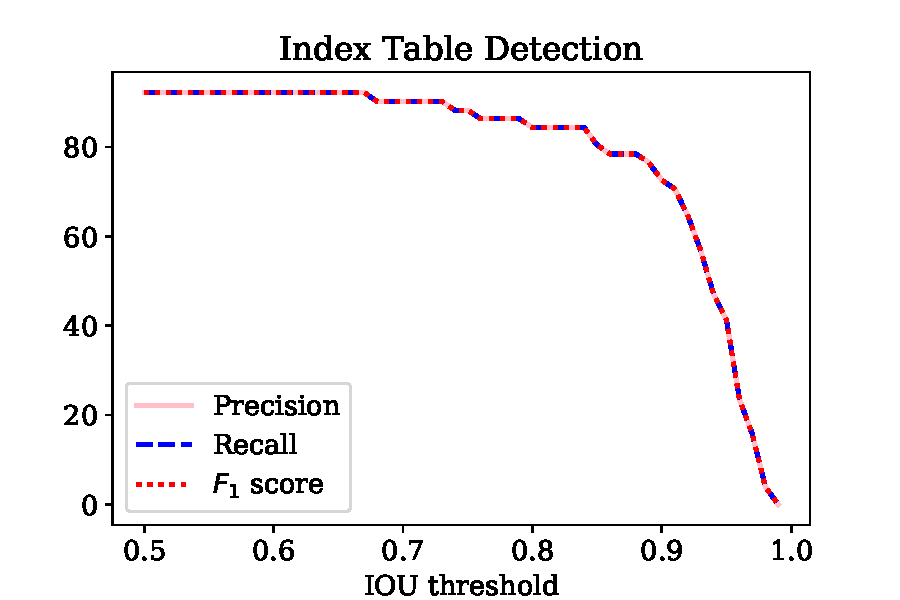
\includegraphics[width=\linewidth]{index_table_pRf.pdf}
    \caption{}
    \label{}
\end{subfigure}
\begin{subfigure}{0.325\linewidth}
  \centering
  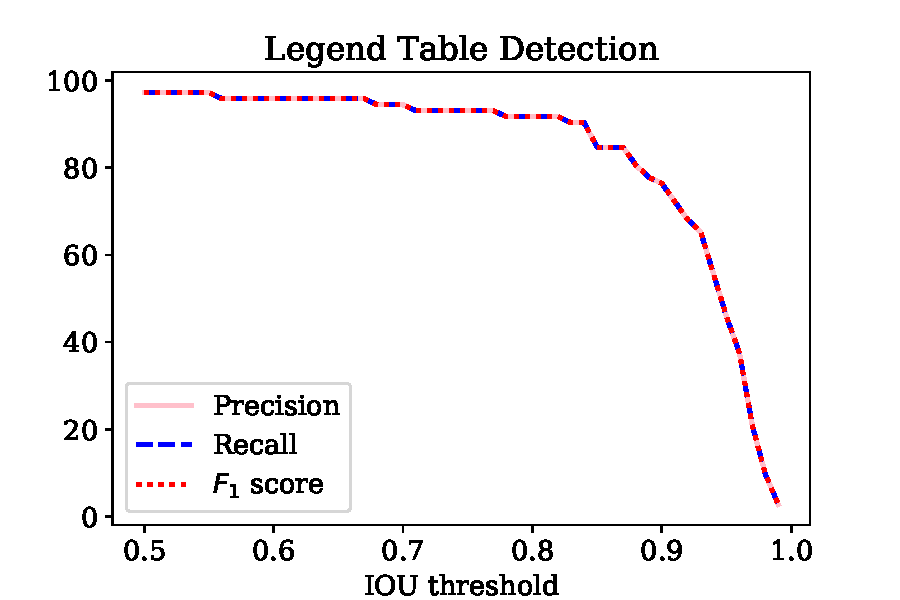
\includegraphics[width=\linewidth]{legend_table_pRf.pdf}
    \caption{}
    \label{}
\end{subfigure}
\caption{Precision, recall and $F_1$ score curves for Legend Tables (C) bends later than Index Tables (B) because dataset contains more number of Legend Tables and less variety of table layouts than Index Tables.}
\label{fig:table_graph}
\end{figure*}
\begin{figure}[!h]
  \centering
  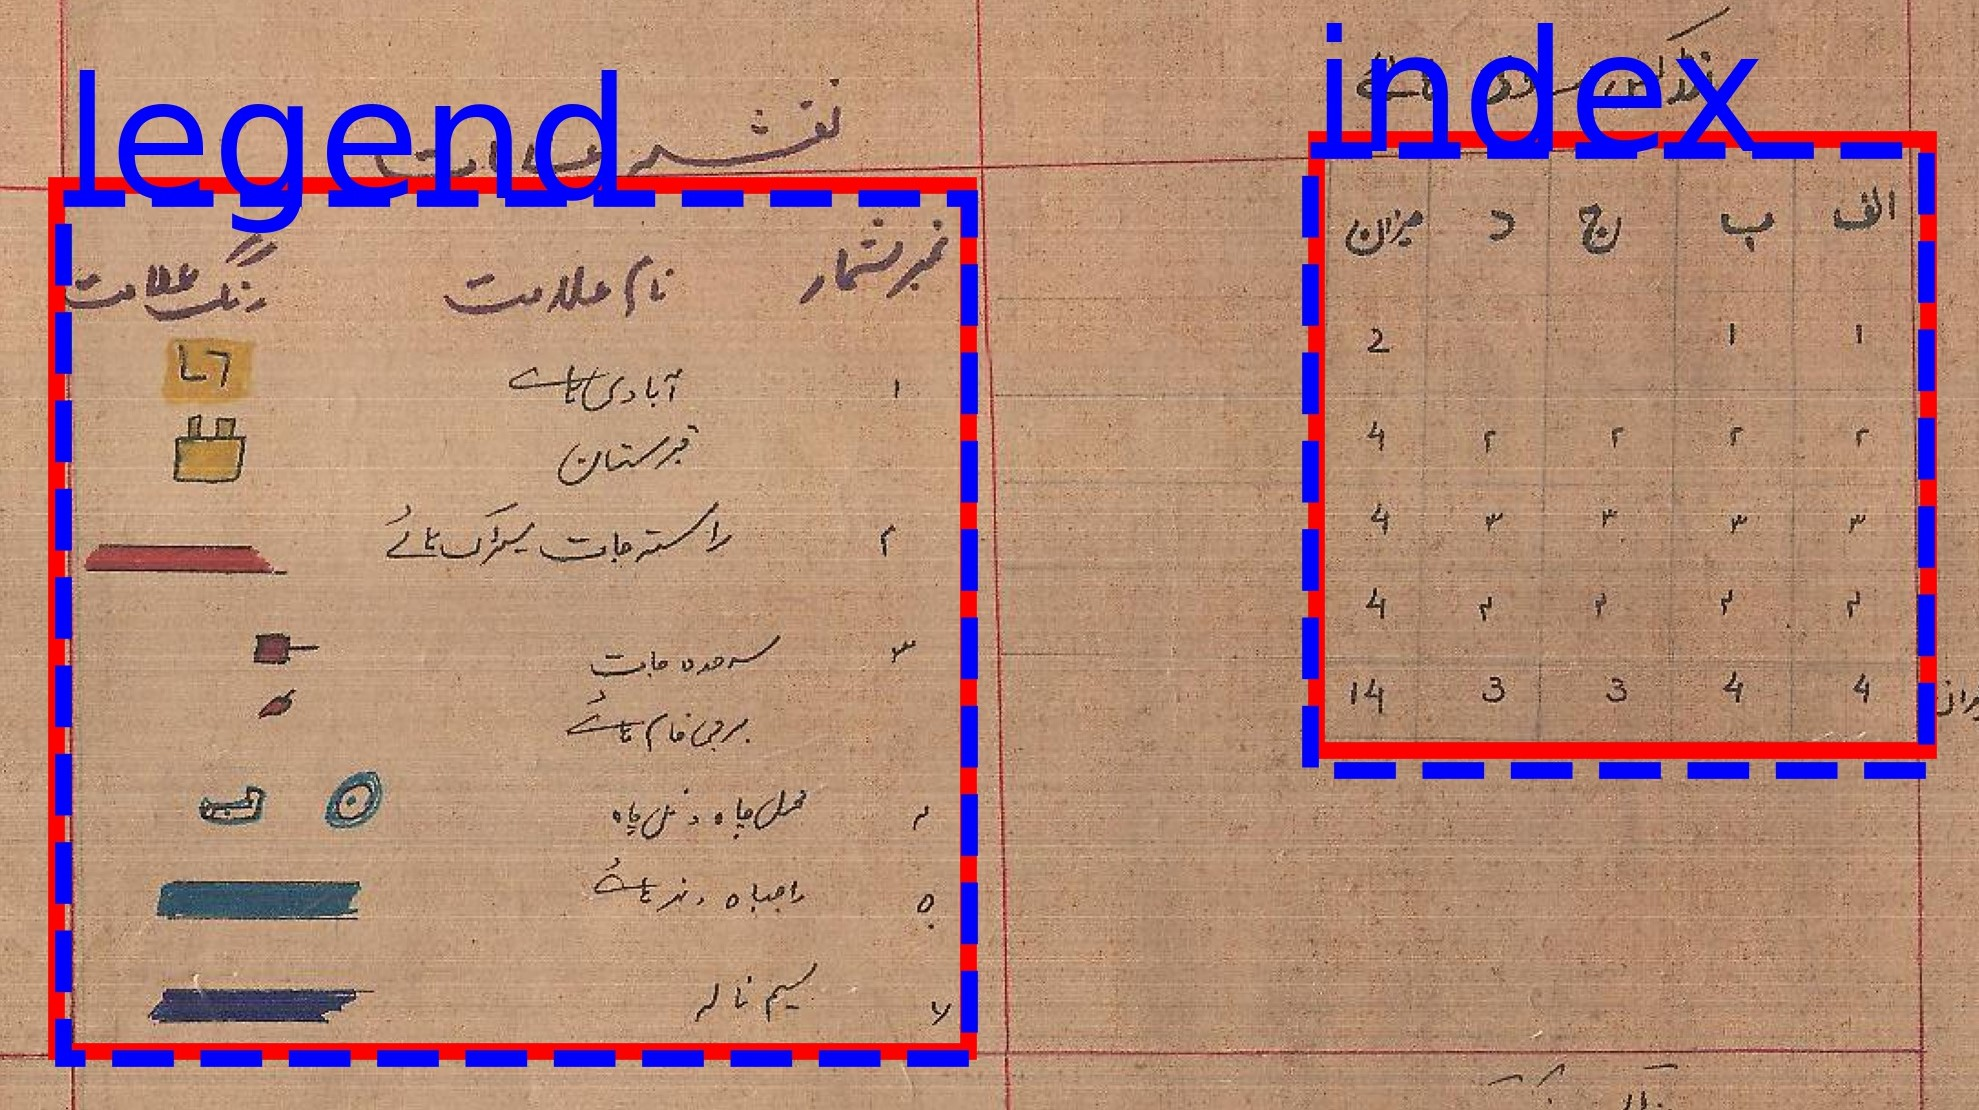
\includegraphics[width=\linewidth,keepaspectratio]{massavi_405 -tables.jpg}
  \caption{Actual tables are represented with red bounding boxes while predicted tables are represented with dashed blue color bounding boxes}
  \label{fig:table_detection}
\end{figure}
\begin{figure}[!h]
\centering
\begin{subfigure}{0.47\linewidth}
  \centering
  % include first image
  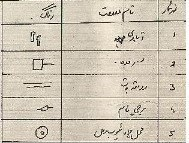
\includegraphics[width=\linewidth,keepaspectratio]{1714 _index.jpg}
    \caption{classified as Index.}
    \label{}
\end{subfigure}
\begin{subfigure}{0.47\linewidth}
  \centering
  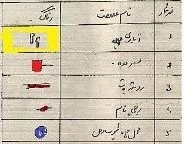
\includegraphics[width=\linewidth,keepaspectratio]{1714 _legend.jpg}
    \caption{classified as Legend.}
    \label{}
\end{subfigure}
\caption{The only misclassified table(A), actually it's a Legend Table, After filling the color in symbols(B) our model classified it as Legend Table. This behavior of model shows that model learns a bias from colourful symbols in Legend Tables to classify these tables as legend.}
\label{fig:missclassified_table}
\end{figure}
\begin{figure*}[h!]
    \centering
    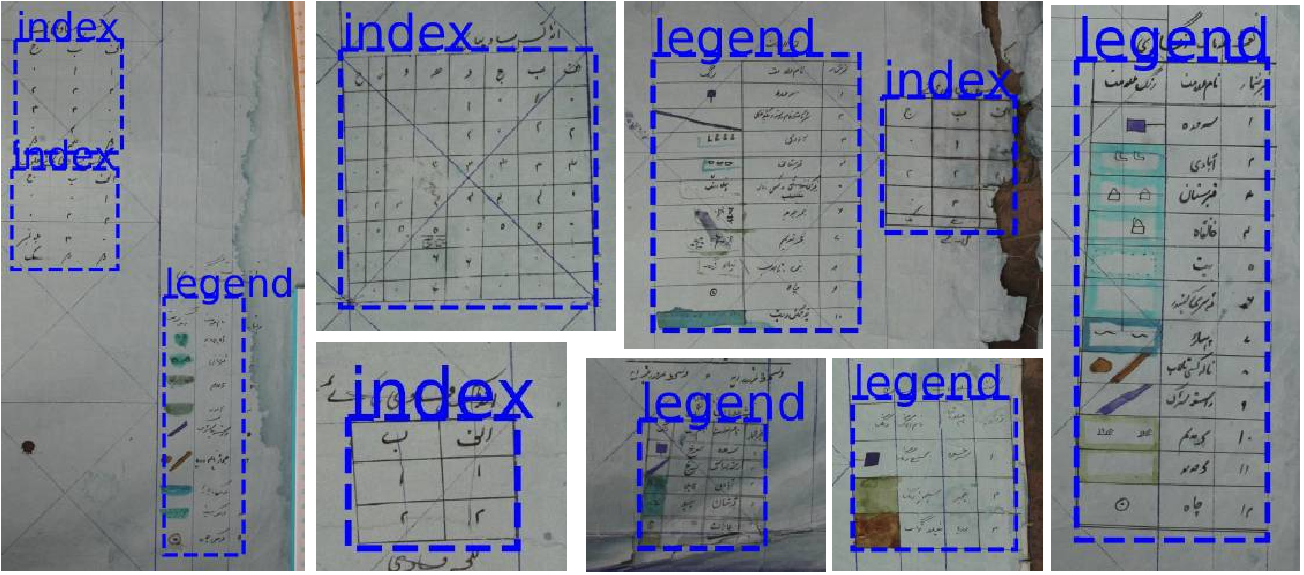
\includegraphics[width=\linewidth, angle=0]{resultOutOfDataset-highQuality.pdf}
    \caption{Table detection results on out of dataset images with variations in layouts among both Index and Legend Tables. In our dataset one map image contain one Index Table. From left first image contain two Index Tables and our model predicted both Index Tables. }
    \label{fig:outOfDataset}
\end{figure*}
Training deep learning models such as Mask R-CNN requires a lot of annotated data which we don't have. So, we have used the concept of domain adaptation and transfer learning to compensate with our small dataset of 356 images. We randomly divided the MapIndexLegendTables dataset with 356 images into two parts with 80:20 ratio, 80 percent data for training while 20 percent of the data for validation. This division resulted in 284 images for training and 72 images for validation. We trained Mask R-CNN model with backbone Resnet-101 architecture. For generating good results on small dataset we initialized Mask R-CNN model with pretrained weights on mscoco dataset. We trained our model for 50 epochs, each epoch with 284 iterations. \autoref{tbl:table_detection} shows numerical results for table detection, separate results for Index Table detection and Legend Table detection. Precision, recall and $F_1$ score values for Index Tables are less than precision, recall and $F_1$ score values for Legend Tables because Index Tables are less in number than Legend Tables and Index Tables are drawn with variety of layouts. One thing to note here is that precision, recall and $F_1$ score values are equal, this happens because False Positives and False Negatives are equal. Graphical representation of precision, recall and $F_1$ score over IoU threshold values ranging from 0.5 to 1.0 with a gap of 0.01 are shown in \autoref{fig:table_graph}. \autoref{fig:table_detection} is showing table detection and classification result on one of the map image from testing data which contains tables with no borders, no horizontal and vertical lines separating rows and columns. We have shown part of the massavi image where tables are located and cropped rest of the content to let the reader focus only on tabular area. Text written in blue is showing the predicted class for each table in the image. Red bounding boxes are ground truths and dashed blue bounding boxes are predicted boxes for tables. All of the tables in map images from testing data are truly classified by our model except one which is shown in \autoref{fig:missclassified_table}.
\begin{figure}[h!]
    \centering
    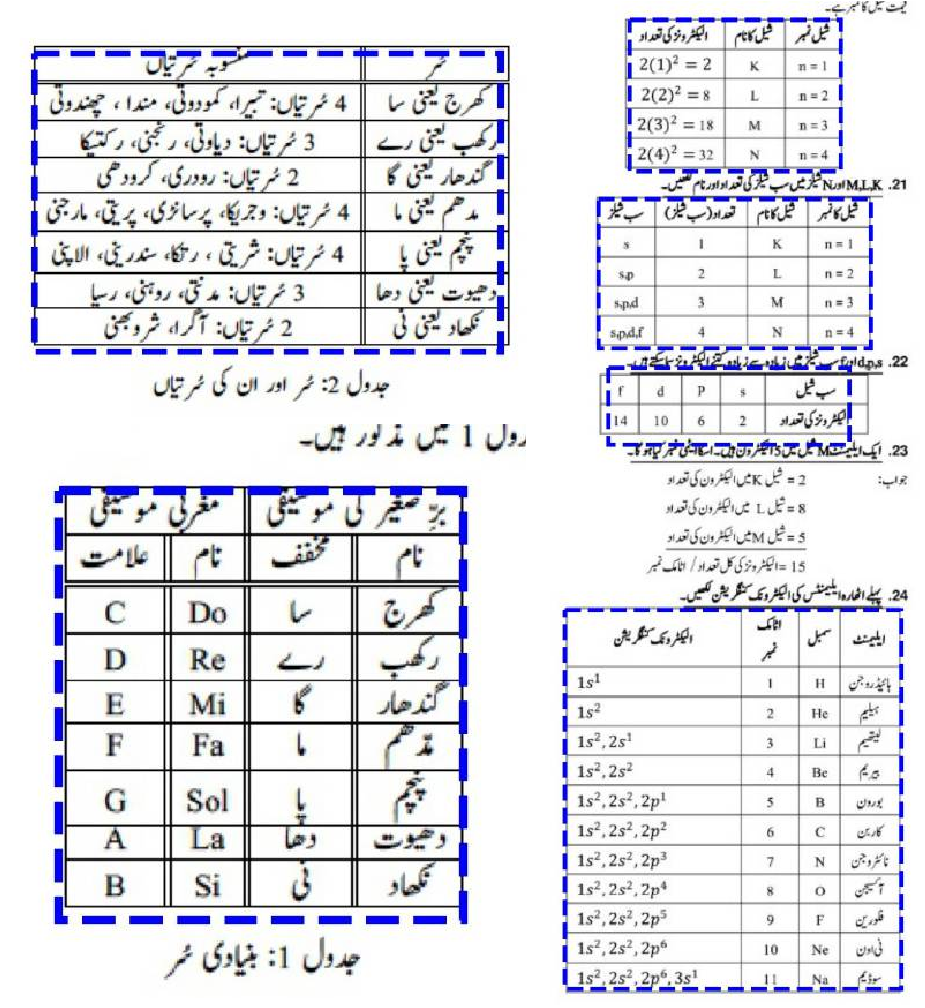
\includegraphics[width=\linewidth, angle=0]{tables_nonMapImages.pdf}
    \caption{Table detection results on non-map images. These images are entirely different than map images. Results show that model does not rely only on content of the table but also on a specific structure that makes a table.}
    \label{fig:nonMapImages}
\end{figure}
\begin{figure}[h!]
    \centering
    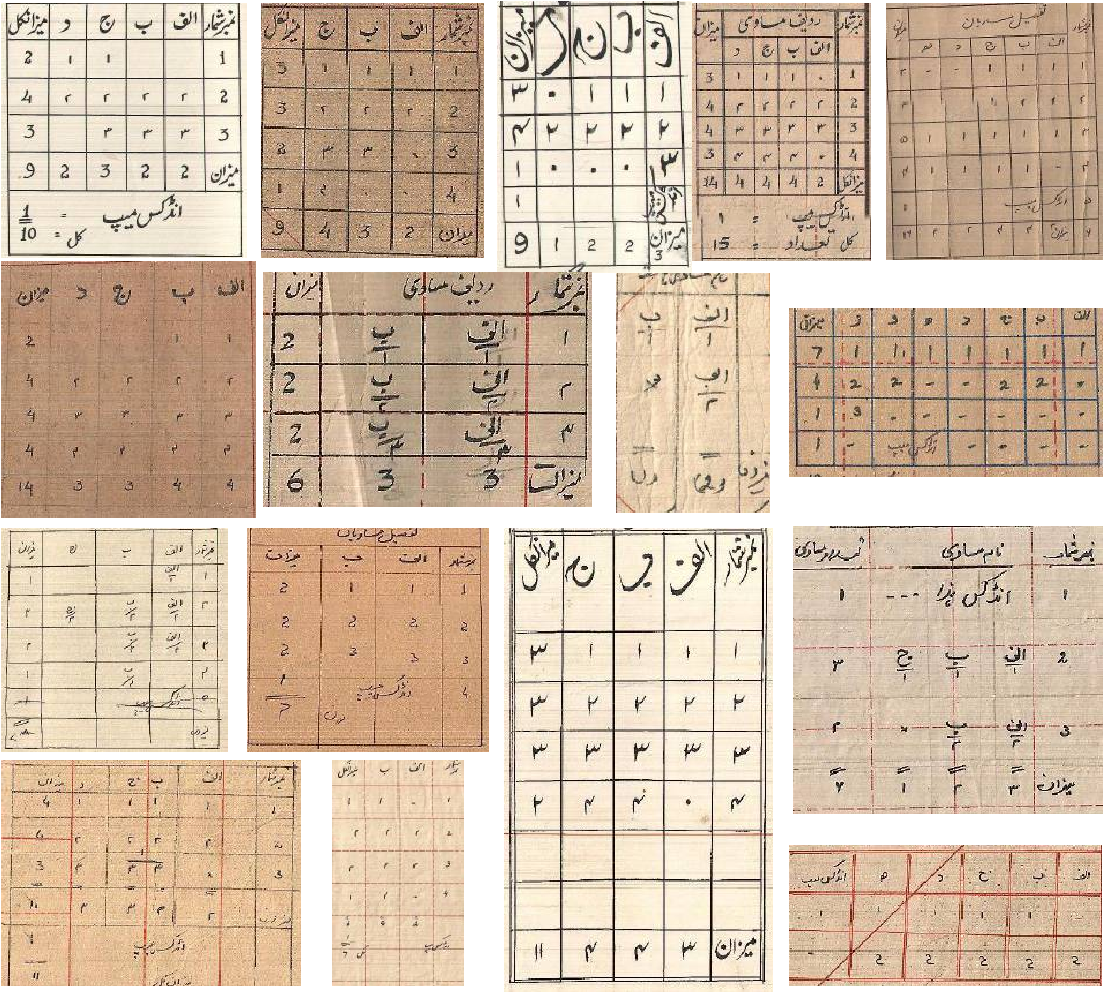
\includegraphics[width=\linewidth, angle=0]{indexTables.pdf}
    \caption{Table detection results by our model on Index Tables with different background colors, complex structure (nested columns, row spanning cells, column spanning cells), background grid lines, variation in layouts, variation in style and font of text, some tables with borders, some tables without borders. Model gives bounding boxes for these tables drawn on map images. We have shown cropped area inside the detected bounding boxes for Index Tables instead of showing the whole map images which are very large as shown in \autoref{fig:masavi}.}
    \label{fig:indexTables}
\end{figure}

\begin{figure}[h!]
    \centering
    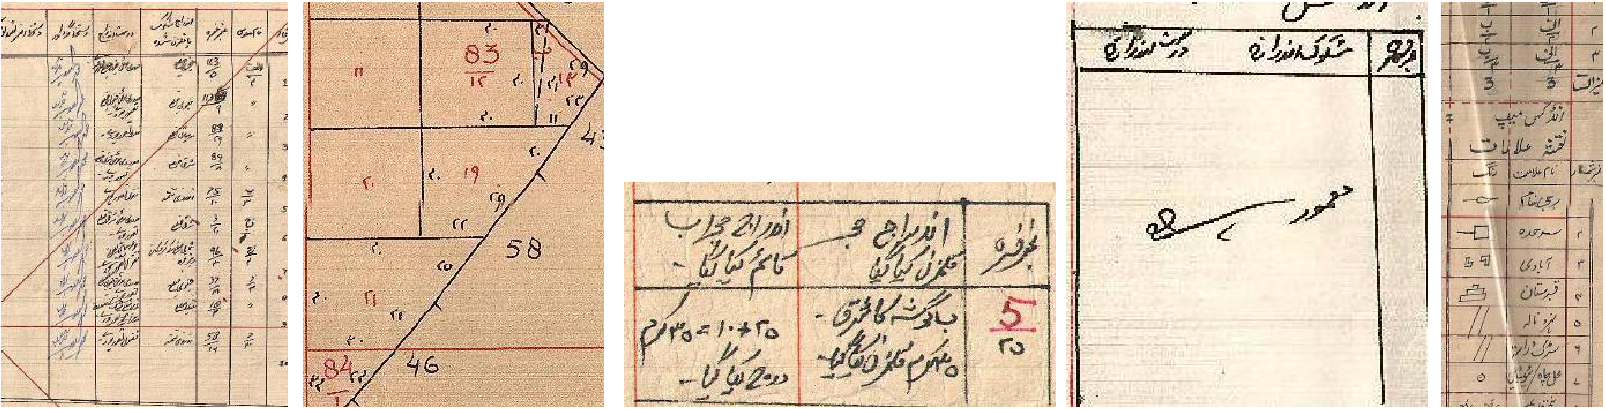
\includegraphics[width=\linewidth, angle=0]{FalsePositiveTables.pdf}
    \caption{False Positive detections by our model, first, third and fourth image from left are actually tabular structures but these are not Index and Legend tables, second image from left is part of map with background grid lines which look like horizontal and vertical lines of a table, fifth and the last image contains Index and Legend Table but both in a single bounding box which is an extra detected box by our model.}
    \label{fig:FalsePositiveTables}
\end{figure}

\begin{figure}[h!]
    \centering
    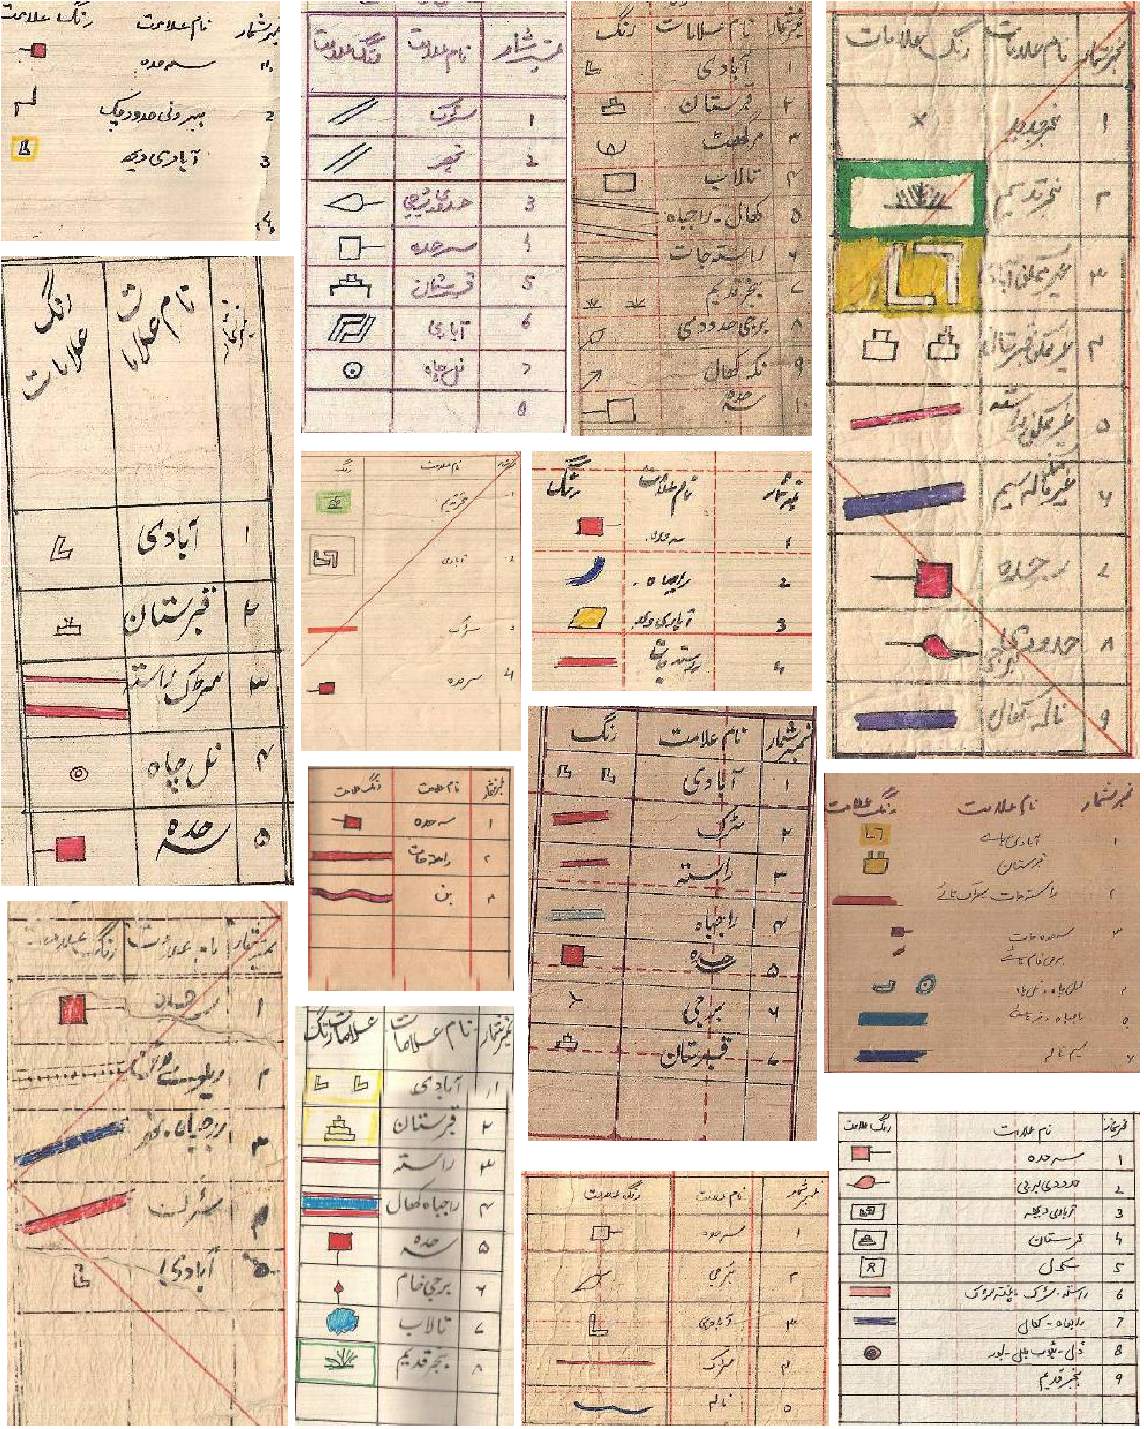
\includegraphics[width=\linewidth, angle=0]{legendTables.pdf}
    \caption{Table detection results by our model on Legend Tables with different background colors, background grid lines, variation in layouts, variation in style and font of text, some tables with borders, some tables without borders. Model gives bounding boxes for these tables drawn on map images. We have shown cropped area inside the detected bounding boxes for Legend Tables instead of showing the whole map images which are very large as shown in \autoref{fig:masavi}.}
    \label{fig:legendTables}
\end{figure}
We have also evaluated our model on out of dataset images. These images have never been seen by the model. Some of the results for these are shown in \autoref{fig:outOfDataset}. These table are truly detected and truly classified. Apart from map images containing tables we have also generated results on map images which do not contain any table and model also predicted no tabular region in these images. This means if model doesn't find any tabular structure in the input image then it gives zero bounding boxes. \autoref{fig:nonMapImages} is showing table detection results on non map images and the predictions are very good. It seems that model doesn't rely only on the content but also on the structure of table for predicting bounding boxes for tables. Table detection results on map images from testing dataset having tables with challenges such as different layouts, complex structures, different background colors, boundary lines, no borders, background grid lines, symbols in Legend Tables sometimes filled with colors and sometimes not, left skewed tables, right skewed tables, varying spacing among rows and columns. One thing to note here is that unlike Legend Tables, Index Tables have nested columns, rows spanning cells and column spanning cells which makes its structure complex. We cropped tables detected by our model from different map images in testing dataset. Index Tables detected by our model are shown in \autoref{fig:indexTables}, and Legend Tables detected by our model are shown in \autoref{fig:legendTables}. False Positive detection by our table detection model are shown in \autoref{fig:FalsePositiveTables}
\subsection{Row and Column Detection}
\label{sec:expResults_rowCol}
\begin{table*}[h!]
\caption{Results for Row and Column Detection}
\label{tbl:row_col_detection}
\centering
\resizebox{\textwidth}{!}{%
\begin{tabular}{| c | c | c |c | c | c |c | c | c |c | }
\hline
&\multicolumn{3}{|c|}{\textbf{IoU=0.5}} &\multicolumn{3}{|c|}{\textbf{IoU=0.75}}& \multicolumn{3}{|c|}{\textbf{IoU=0.9}}\\
\hline
 &\textbf{P@0.5} & \textbf{R@0.5}  & \textbf{$F_1$@0.5} & \textbf{P@0.75} & \textbf{R@0.75}  & \textbf{$F_1$@0.75}& \textbf{P@0.9} & \textbf{R@0.9}  & \textbf{$F_1$@0.9} \\ 
 \hline
\multicolumn{10}{|c|}{\textbf{Combined Results on both Index and Legend Tables}}\\
 \hline
 \textbf{Row and Column Detection} & 97.0\% & 97.59\% & 97.29\% & 92.35\% & 92.91\% & 92.63\% & 62.37\% & 62.75\% & 62.56\% \\
 \hline
 \textbf{Row Detection} & 96.55\% & 97.45\% & 97.0\% & 93.56\% & 94.43\% & 94.0\% & 74.02\% & 74.71\% & 74.36\%\\
 \hline
 \textbf{Column Detection} & 97.84\% & 97.84\% & 97.84\% & 90.09\% & 90.09\% & 90.09\% & 40.52\% & 40.52\% & 40.52\%\\
  \hline
\multicolumn{10}{|c|}{\textbf{Results on Index Tables}}\\
 \hline
 \textbf{Row and Column Detection} & 93.16\% & 95.7\% & 94.41\% & 86.31\% & 88.67\% & 87.48\% & 57.79\% & 59.38\% & 58.57\% \\
 \hline
 \textbf{Row Detection} & 90.71\% & 95.49\% & 93.04\% & 87.14\% & 91.73\% & 89.38\% & 70.0\% & 73.68\% & 71.79\% \\
 \hline
 \textbf{Column Detection} & 95.93\% & 95.93\% & 95.93\% & 85.37\% & 85.37\% & 85.37\% & 43.9\% & 43.9\% & 43.9\% \\
 \hline
\multicolumn{10}{|c|}{\textbf{Results on Legend Tables}}\\
 \hline
 \textbf{Row and Column Detection} & 99.5\% & 98.77\% & 99.14\% & 96.29\% & 95.58\% & 95.93\% & 65.35\% & 64.86\% & 65.1\% \\
 \hline
 \textbf{Row Detection} & 99.32\% & 98.32\% & 98.82\% & 96.61\% & 95.64\% & 96.12\% & 75.93\% & 75.17\% & 75.55\% \\
 \hline
 \textbf{Column Detection} & 100.0\% & 100.0\% & 100.0\% & 95.41\% & 95.41\% & 95.41\% & 36.7\% & 36.7\% & 36.7\% \\
 \hline
\multicolumn{10}{|c|}{\textbf{Results on Legend Tables}}\\
\multicolumn{10}{|c|}{\textbf{(by the model pretrained on both index and legend tables, then trained specifically on Legend Tables)}}\\
 \hline
 \textbf{Row and Column Detection} & 99.75\% & 99.51\% & 99.63\% & 97.29\% & 97.05\% & 97.17\% & 72.66\% & 72.48\% & 72.57\% \\
 \hline
 \textbf{Row Detection} & 99.66\% & 99.33\% & 99.5\% & 97.31\% & 96.98\% & 97.14\% & 73.06\% & 72.82\% & 72.94\% \\
 \hline
 \textbf{Column Detection} & 100.0\% & 100.0\% & 100.0\% & 97.25\% & 97.25\% & 97.25\% & 71.56\% & 71.56\% & 71.56\% \\
 \hline
\end{tabular}
}
\end{table*}
\begin{figure*}[h!]
\centering
\begin{subfigure}{0.325\linewidth}
  \centering
  % include first image
  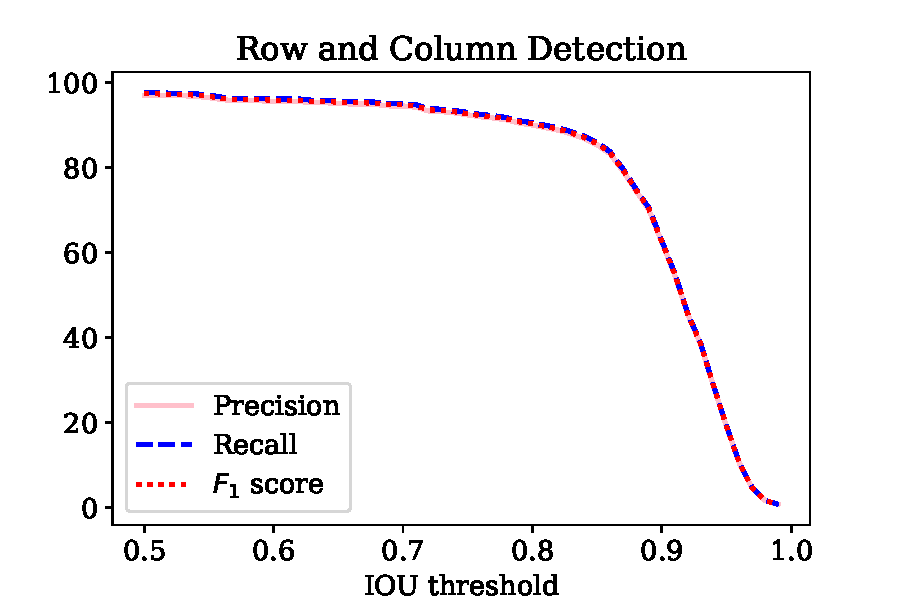
\includegraphics[width=\linewidth]{row_col_pRf.pdf}
    \caption{}
    \label{}
\end{subfigure}
\begin{subfigure}{0.325\linewidth}
  \centering
  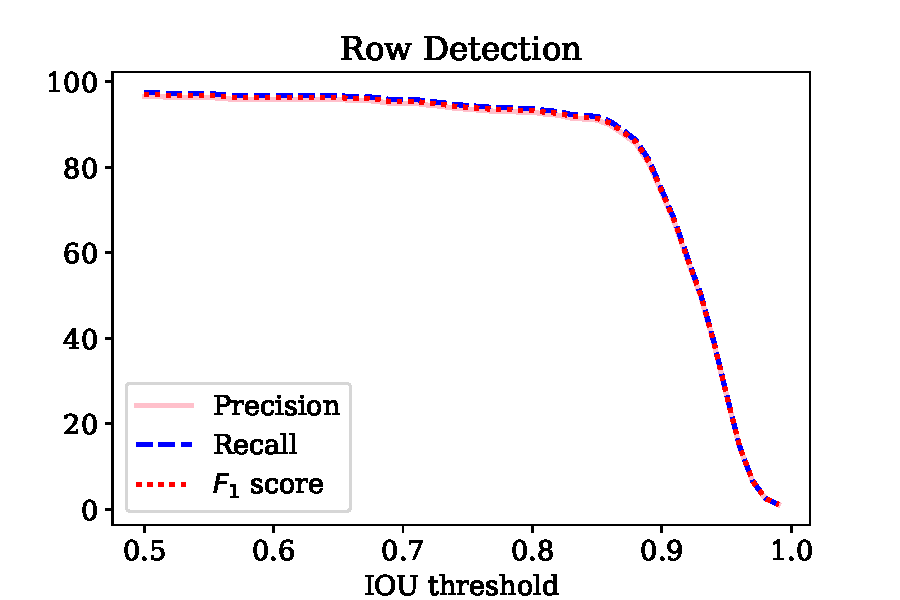
\includegraphics[width=\linewidth]{row_pRf.pdf}
    \caption{}
    \label{}
\end{subfigure}
\begin{subfigure}{0.325\linewidth}
  \centering
  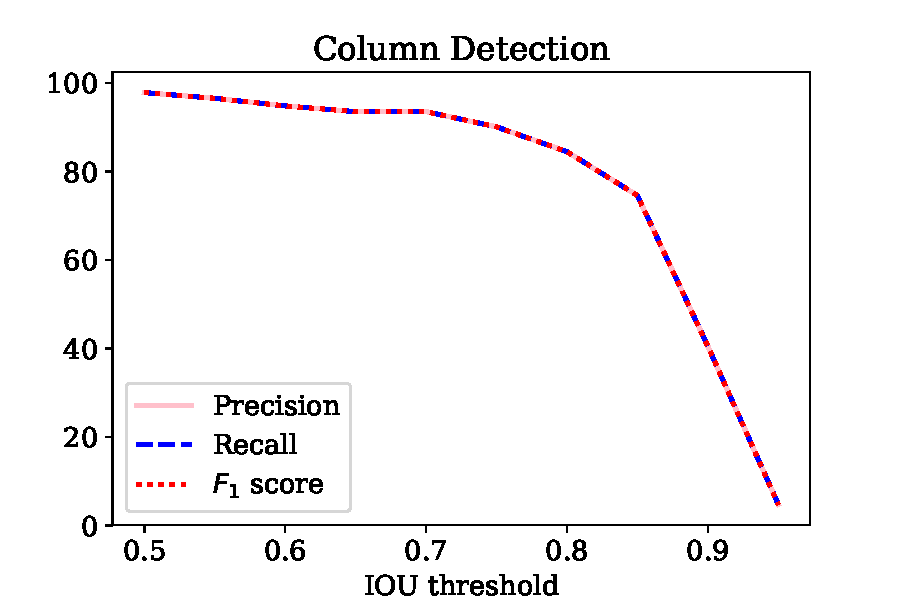
\includegraphics[width=\linewidth]{col_pRf.pdf}
    \caption{}
    \label{}
\end{subfigure}
\caption{(A) shows combined results for rows and columns which falls below 90\% after 0.8 IoU threshold. Precision, recall and $F_1$ score curves for row detection (B) falls very slowly till 0.85 threshold and then falls very fast after 0.9 threshold and touches zero later than column detection (C) whose curves bend gradually with IoU threshold. Model is more accurate in giving bounding boxes values for rows.}
\label{fig:rowCol_graph}
\end{figure*}
For detection of rows and columns we prepared MapTablesRowCol dataset which we introduced in section 4.1. This dataset contains 616 images of tables. We randomly split it into three parts with 80:10:10 ratio. We used 80 percent data for training which are 495 images of tables. 10 percent data which are 61 images from dataset are used for validation while the remaining 10 percent, 60 images are used for testing. We used pretrained weights of Mask R-CNN on mscoco dataset as the starting point and then trained on our dataset.
\begin{figure*}[h!]
  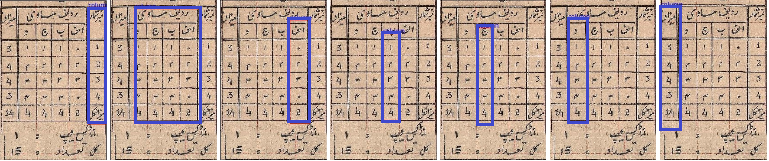
\includegraphics[width=\linewidth]{column_index_144_edited.png}
  \caption{Detected columns in an Index Table. Second blue box from left is a super column with three sub columns which are shown subsequently in the same figure. This shows that model can detect nested columns as well.}
  \label{fig:colindex}
\end{figure*}
\begin{figure*}[h!]
  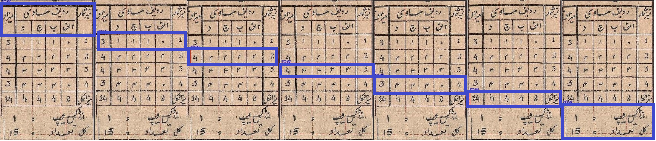
\includegraphics[width=\linewidth]{rows_index_144_edited.png}
  \caption{Detected rows in an Index Table.}
  \label{fig:rowindex}
\end{figure*}
We run the experiment for 495 iterations and 13 epochs. Numerical results for row and column detection are shown in \autoref{tbl:row_col_detection}, at 0.5 IoU threshold precision, recall and $F_1$ score values for row detection are less than precision, recall and $F_1$ score values for column detection which means that there is more False Positive and False Negative rate in detecting rows, but as we increase IoU threshold precision, recall and $F_1$ score values for row detection beats precision, recall and $F_1$ score values for column detection keeping the same threshold which concludes that model is more good at predicting columns but more accurate at giving bounding box values for rows. This behavior of model is reflected in all of the four sections in \autoref{tbl:row_col_detection}. Among results on Index and Legend Tables precision, recall and $F_1$ score values are higher for Legend Tables because Legend Tables contain more number of rows and columns than Index Tables and structure of Legend Tables is not much complex unlike Index Tables. For column detection results on Legend Tables, at smaller IoU threshold values precision, recall and $F_1$ score values are very 100\% but as we increase IoU threshold to 0.95, precision, recall and $F_1$ score value decrease down to 36.7\%, Legend Tables \autoref{fig:legendTables} have simple structure, there are neither nested column, nor row and column spanning cells still bounding box values given by the model for columns of Legend Tables are not so accurate, this is because of complex structure (nested columns) of Index Tables \autoref{fig:colindex} due to which model learns a bias. We improved  bounding box value accuracies for columns of Legend Tables discussed in section 4.3.2.1 and numerically this improvement is shown in \autoref{tbl:row_col_detection} where precision, recall and $F_1$ score values increase from 36.7\% to 71.56\% at 0.9 IoU threshold. Graphical representation of precision, recall and $F_1$ score for structure recognition of both Index and Legend Tables are shown in \autoref{fig:rowCol_graph}, comparison of row detection results among Index and Legend Tables are shown in \autoref{fig:row_index_legend_graph} and comparison of column detection results among Index and Legend Tables are shown in \autoref{fig:Col_index_legend_graph} .
\begin{figure}[h!]
\centering
\begin{subfigure}{0.48\linewidth}
  \centering
  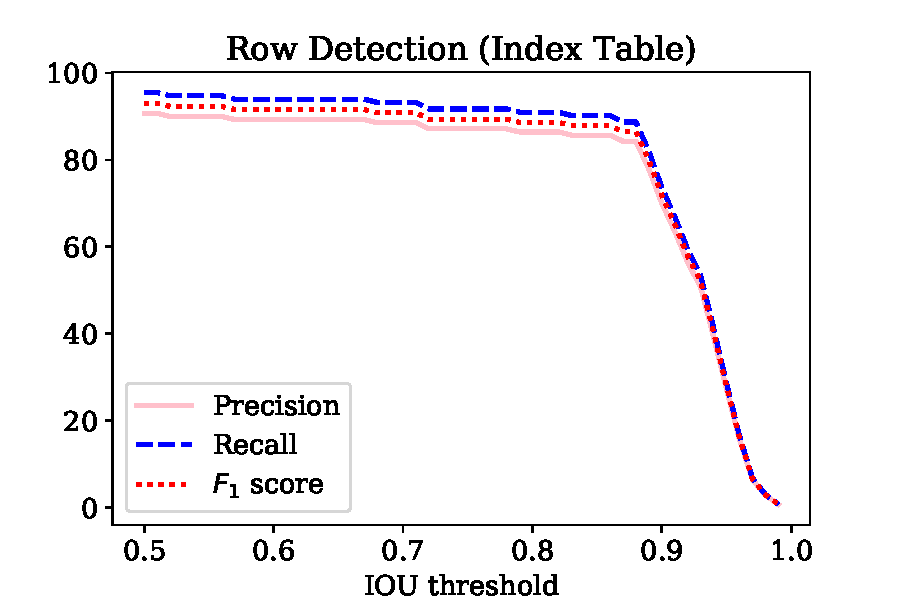
\includegraphics[width=\linewidth]{row_index_pRf.pdf}
    \caption{}
    \label{}
\end{subfigure}
\begin{subfigure}{0.48\linewidth}
  \centering
  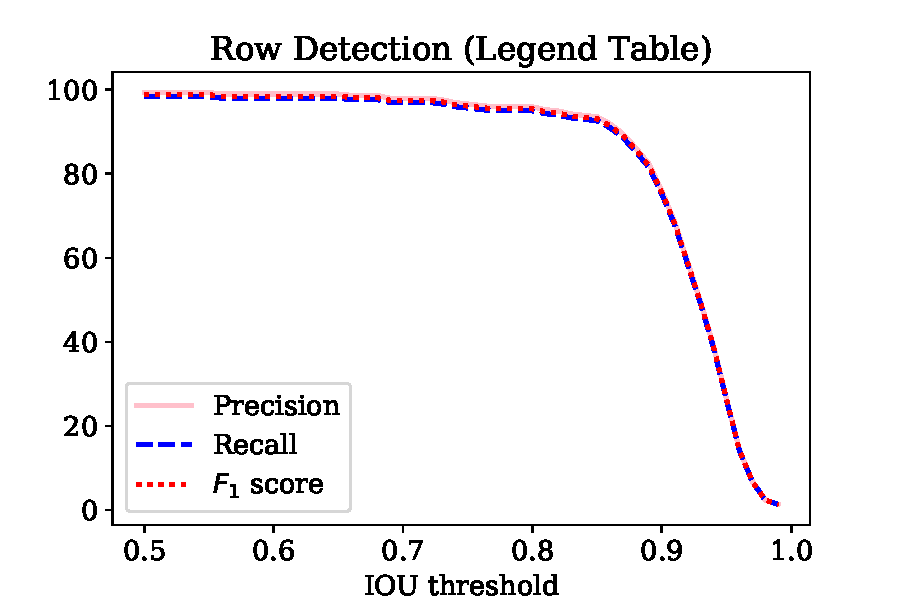
\includegraphics[width=\linewidth]{row_legend_pRf.pdf}
    \caption{}
    \label{}
\end{subfigure}
\caption{Less number of rows in Index Tables as compared to number of rows in Legend Tables tends precision, recall and $F_1$ score curves bends earlier at lower thresholds in (A).}
\label{fig:row_index_legend_graph}
\end{figure}

\begin{figure}[h!]
\centering
\begin{subfigure}{0.48\linewidth}
  \centering
  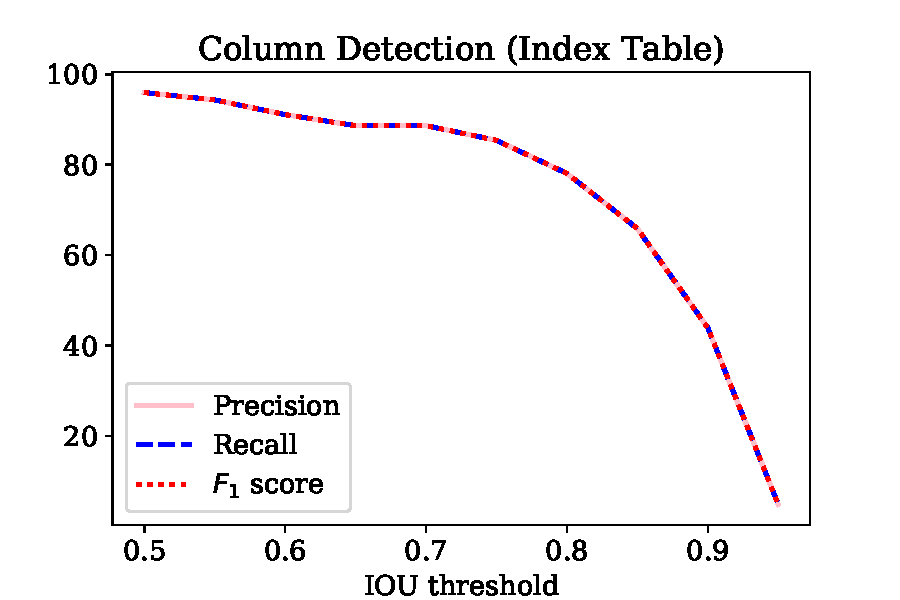
\includegraphics[width=\linewidth]{col_index_pRf.pdf}
    \caption{}
    \label{}
\end{subfigure}
\begin{subfigure}{0.48\linewidth}
  \centering
  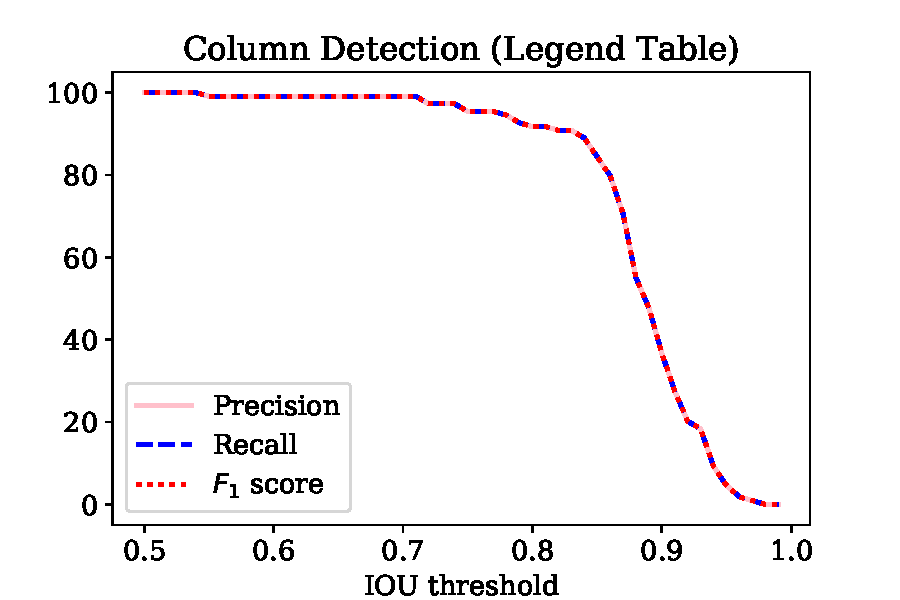
\includegraphics[width=\linewidth]{col_legend_pRf.pdf}
    \caption{}
    \label{}
\end{subfigure}
\caption{Effect of nested columns in Index Tables on column detection results in Legend Tables(B). precision, recall and $F_1$ score curves abruptly falls down at 0.9 IoU threshold.}
\label{fig:Col_index_legend_graph}
\end{figure}
See \autoref{fig:rowindex} for detected rows in an Index Table and \autoref{fig:colindex} for detected column in the same table. There are nested columns in this table and our model detected all these columns. Due to these Index Tables which contains nested columns, model learns a bias and it effects Legend Tables which are very regular and clean in nature. This effect is shown in \autoref{fig:compRowColLegend}(A) in which bounding boxes for columns are not aligned.
\subsubsection{Improved results on Legend Tables for Row and Column Detection}
\label{sec:expResults_rowCol_improved}
\begin{figure}[h!]
\centering
\begin{subfigure}{0.47\linewidth}
  \centering
  % include first image
  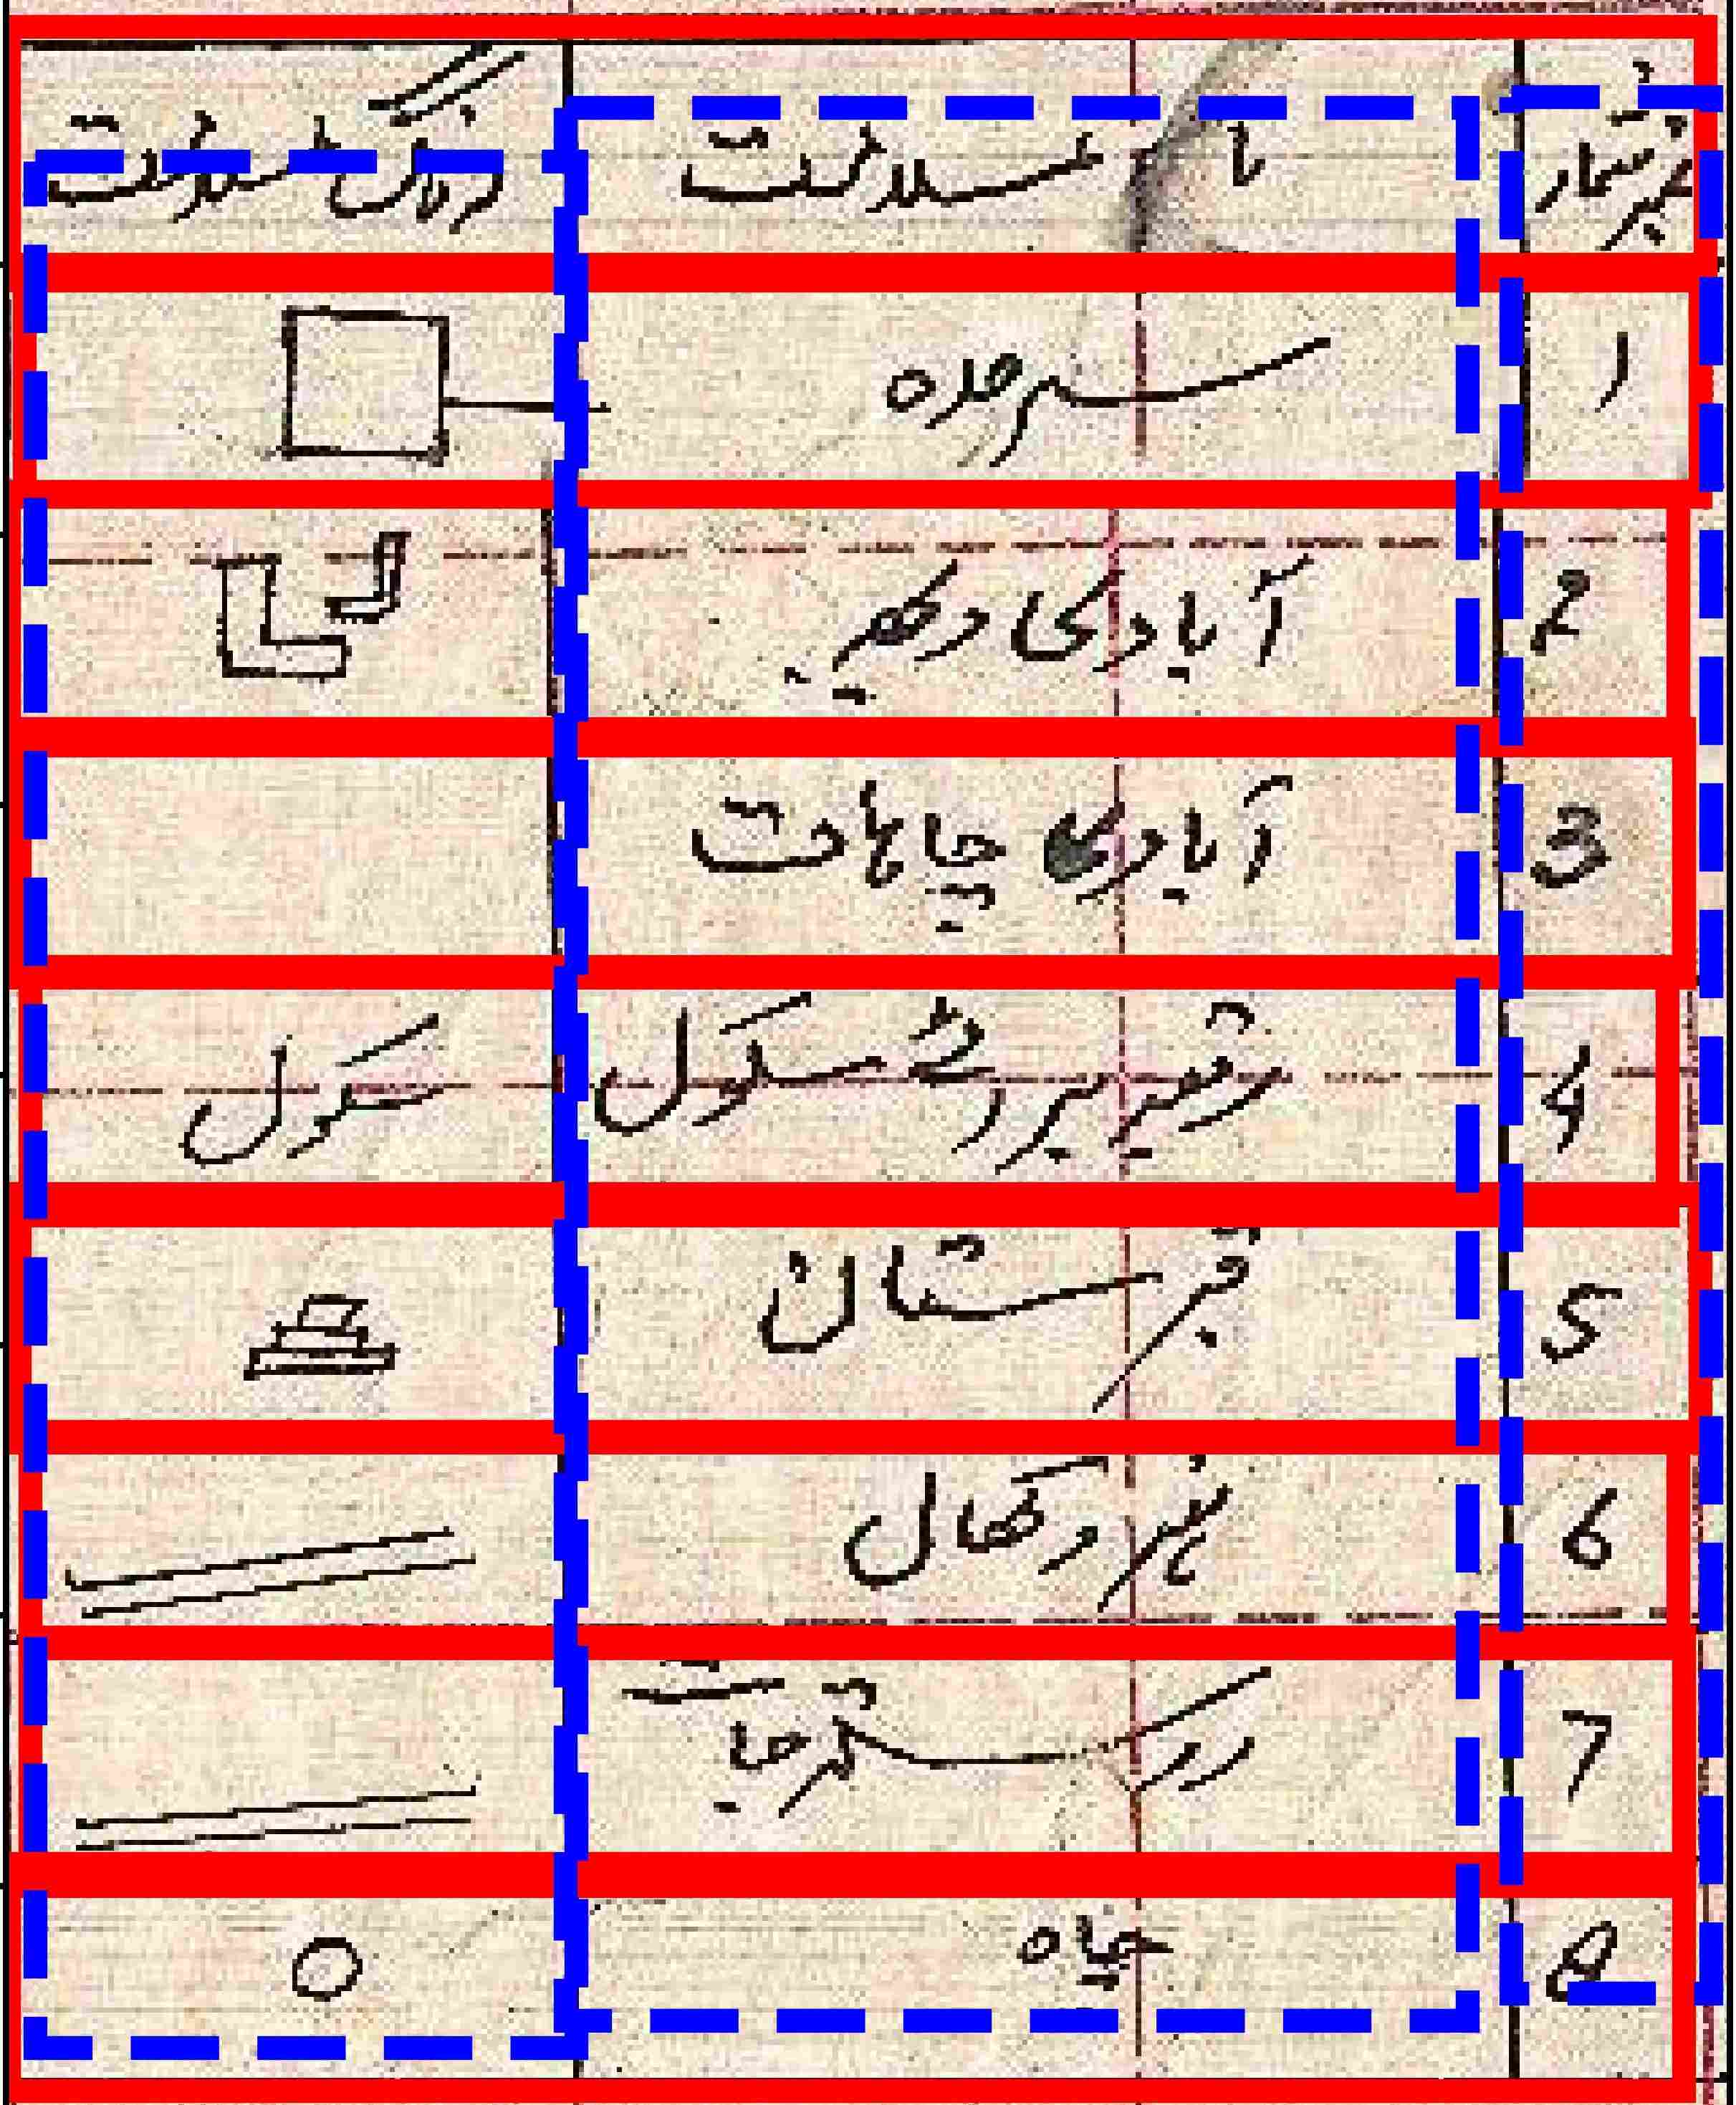
\includegraphics[width=\linewidth]{rowCol_1483_legend.jpg}
    \caption{}
    \label{}
\end{subfigure}
\begin{subfigure}{0.47\linewidth}
  \centering
  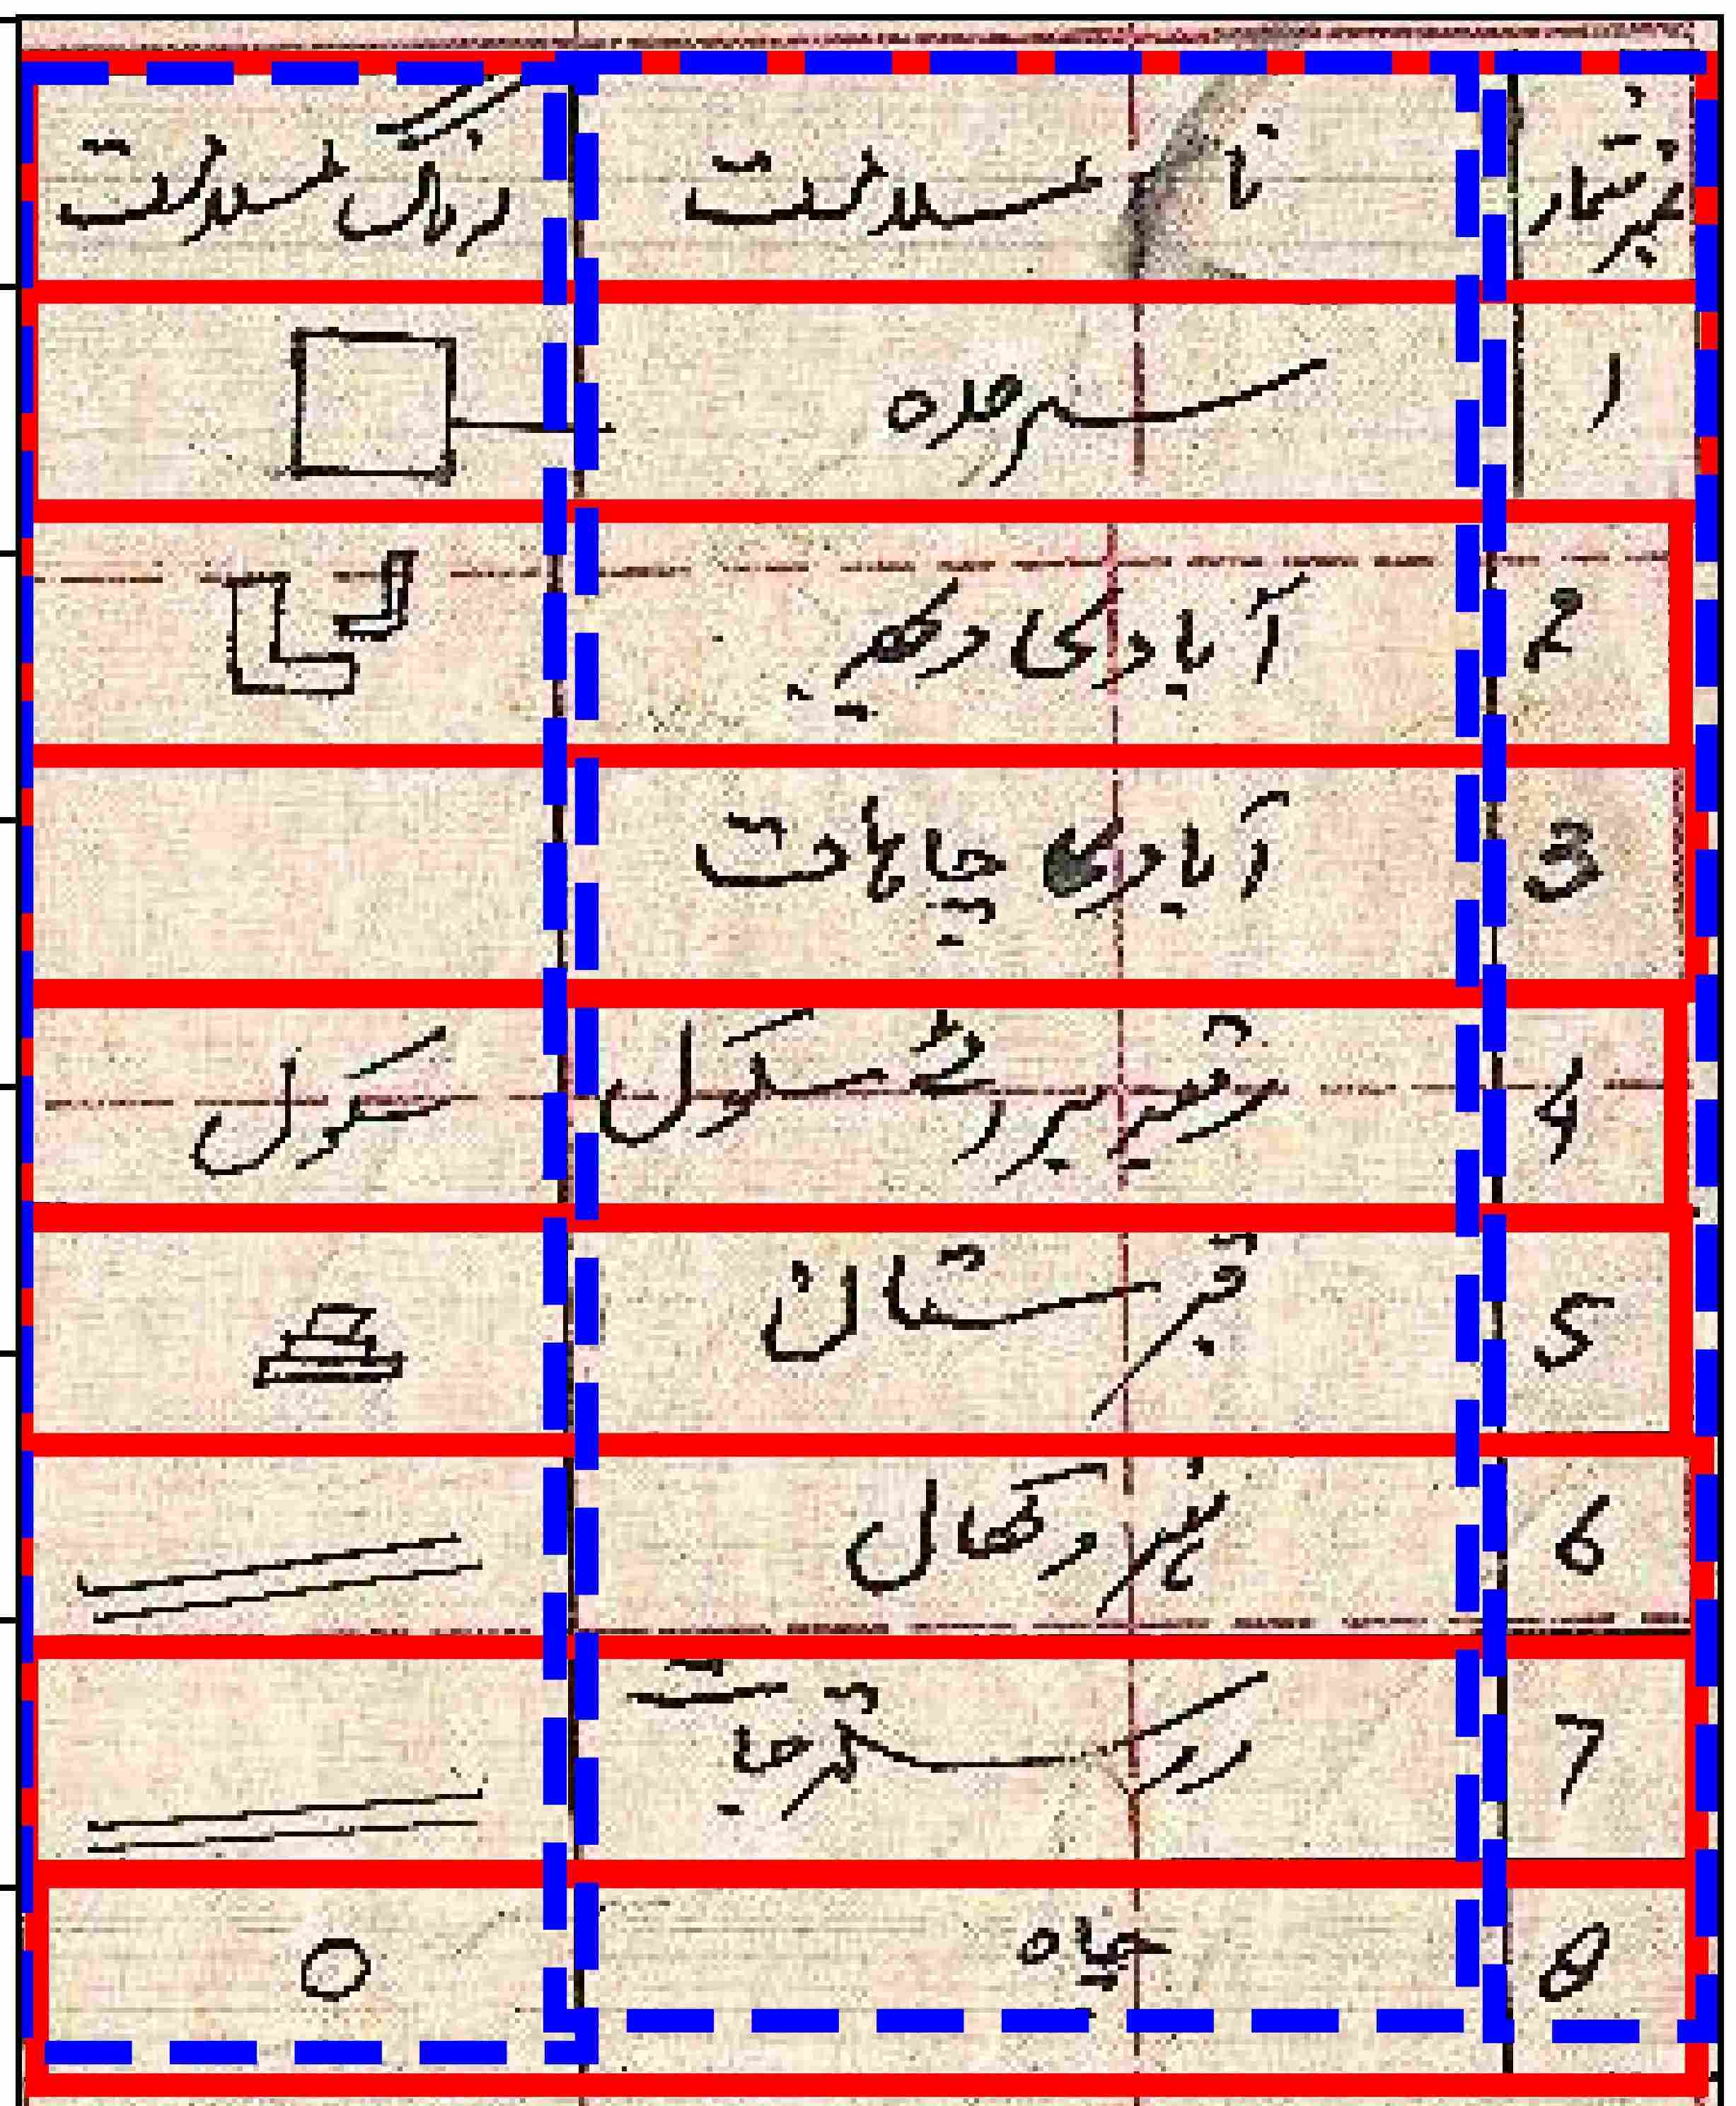
\includegraphics[width=\linewidth]{rowCol_1483__legend_improved.jpg}
    \caption{}
    \label{}
\end{subfigure}
\caption{(a) is showing results for rows and columns which are detected by Mask R-CNN model trained on rows and columns of both Index and Legend tables (b) is showing rows and columns which are detected by Mask R-CNN model initialized with pretrained weights on both Index and Legend tables and then trained specifically on Legend Tables. Bounding boxes for Columns in (B) are more accurate and aligned than in (A).}
\label{fig:compRowColLegend}
\end{figure}
Model is initialized with pretrained weights of row and column detection for both Index and Legend Table exploiting the concept of transfer learning to train model specifically on Legend Tables because they do not contain nested columns, row spanning and column spanning cells unlike Index Tables. \autoref{fig:rowCol_legend_improved_graph} shows a comparison between old and new improved results on column detection in Legend Tables. More accurate results for bounding box values of columns in Legend Tables given by new trained model are shown in \autoref{fig:compRowColLegend}(B).
\begin{figure}[h!]
\centering
\begin{subfigure}{0.48\linewidth}
  \centering
  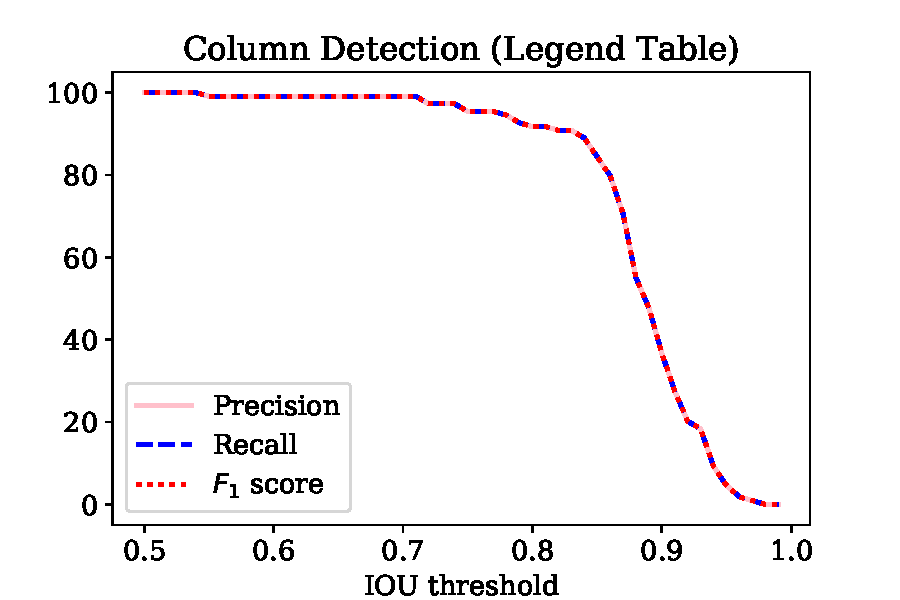
\includegraphics[width=\linewidth]{col_legend_pRf.pdf}
    \caption{}
    \label{}
\end{subfigure}
\begin{subfigure}{0.48\linewidth}
  \centering
  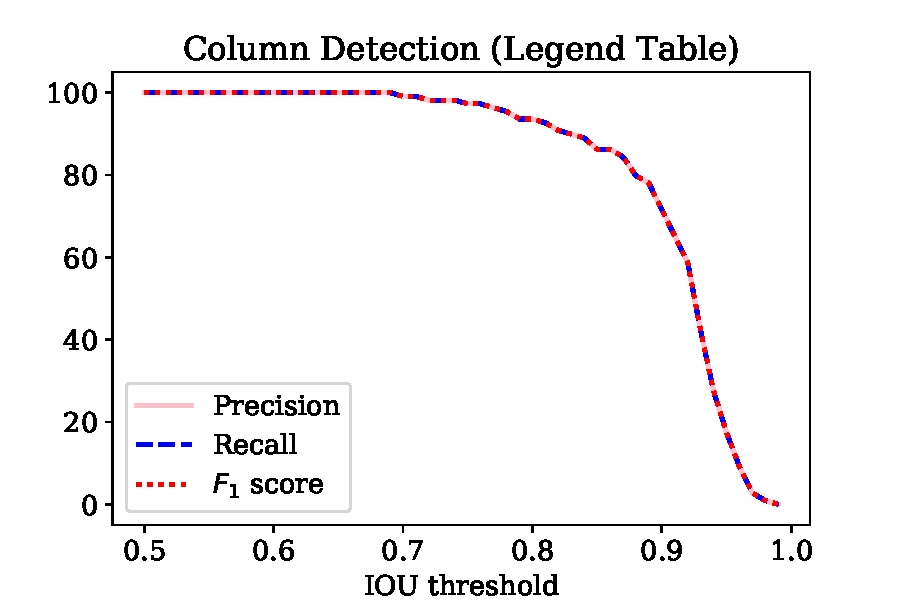
\includegraphics[width=\linewidth]{col_legend_improved_pRf.pdf}
    \caption{}
    \label{}
\end{subfigure}
\caption{(A) shows precision, recall and $F_1$ score curves drawn using model weights trained on rows and columns of both Index and Legend Tables, these curves bends earlier and touches zero earlier while in (B) precision, recall and $F_1$ score curves bend later and touches zero later.}
\label{fig:rowCol_legend_improved_graph}
\end{figure}
\subsubsection{Detection Vs Instance Segmentation}
\label{sec:expResults_instanceSeg}
Detection gives bounding boxes for rows and columns which are horizontal and vertical rectangles. See \autoref{fig:detVsIns}(a) table is not orthogonal rather it is drawn at some angle due to which detection bounding boxes overlaps and we need instance segmentation to have pixel wise masks to uniquely identify each row and column. Results for instance segmentation for rows and columns are shown separately in (b) and (c) respectively for better visibility.

\begin{figure}[h!]
\centering
\begin{subfigure}{0.325\linewidth}
  \centering
  % include first image
  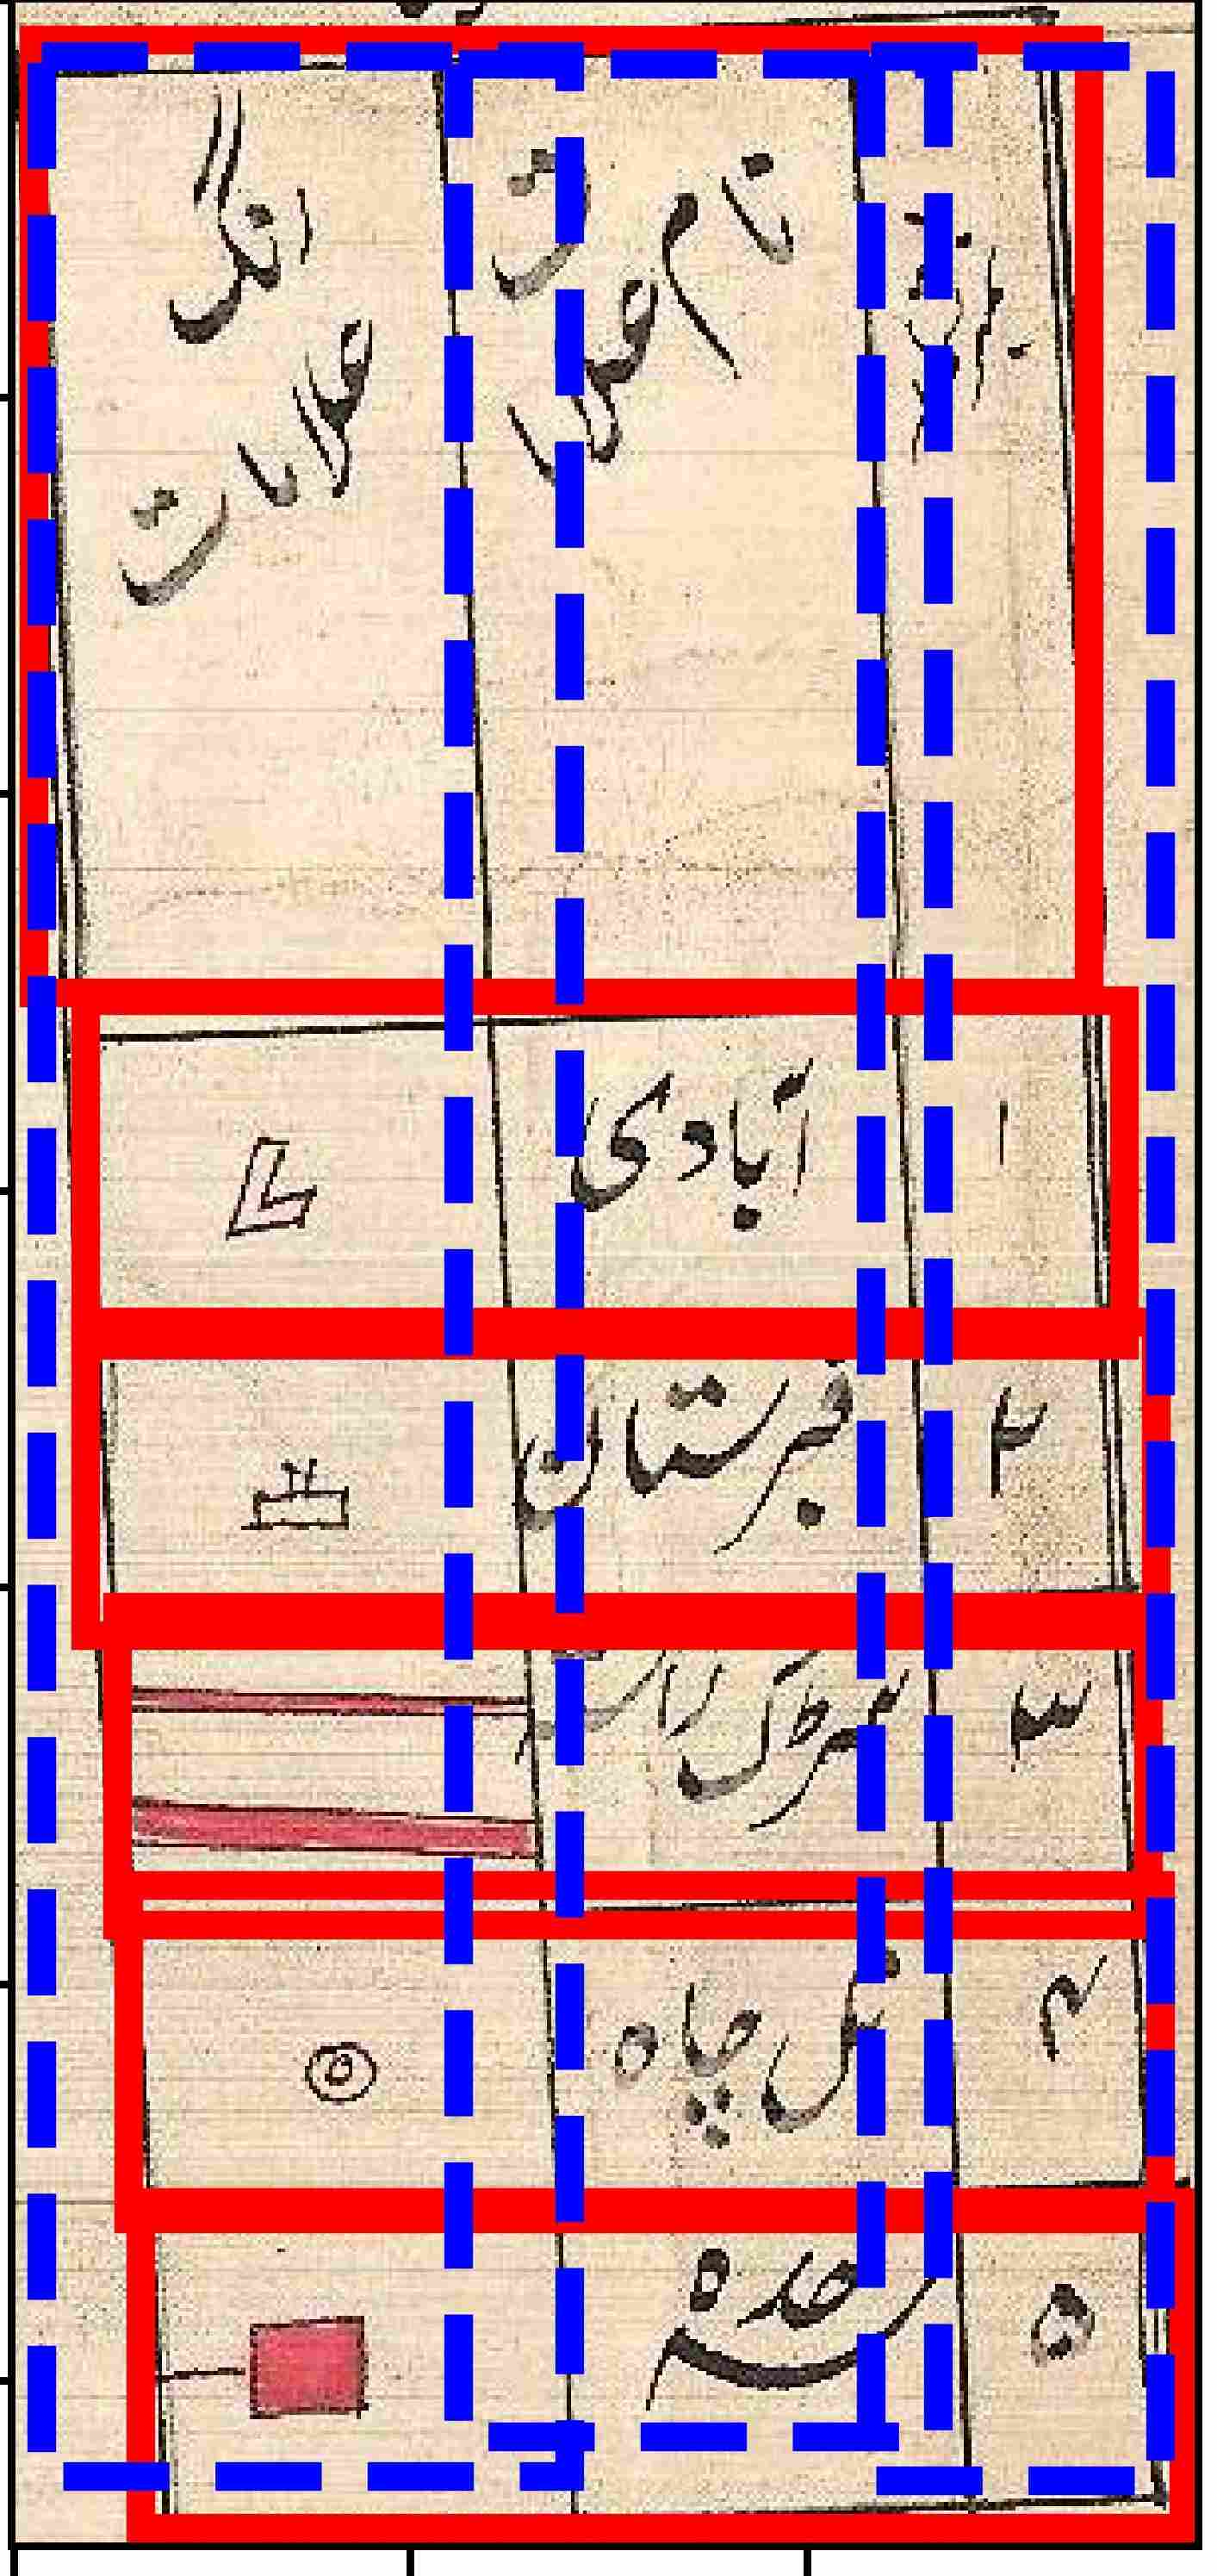
\includegraphics[width=\linewidth]{detection_massavi_1525.jpg}
    \caption{}
    \label{}
\end{subfigure}
\begin{subfigure}{0.325\linewidth}
  \centering
  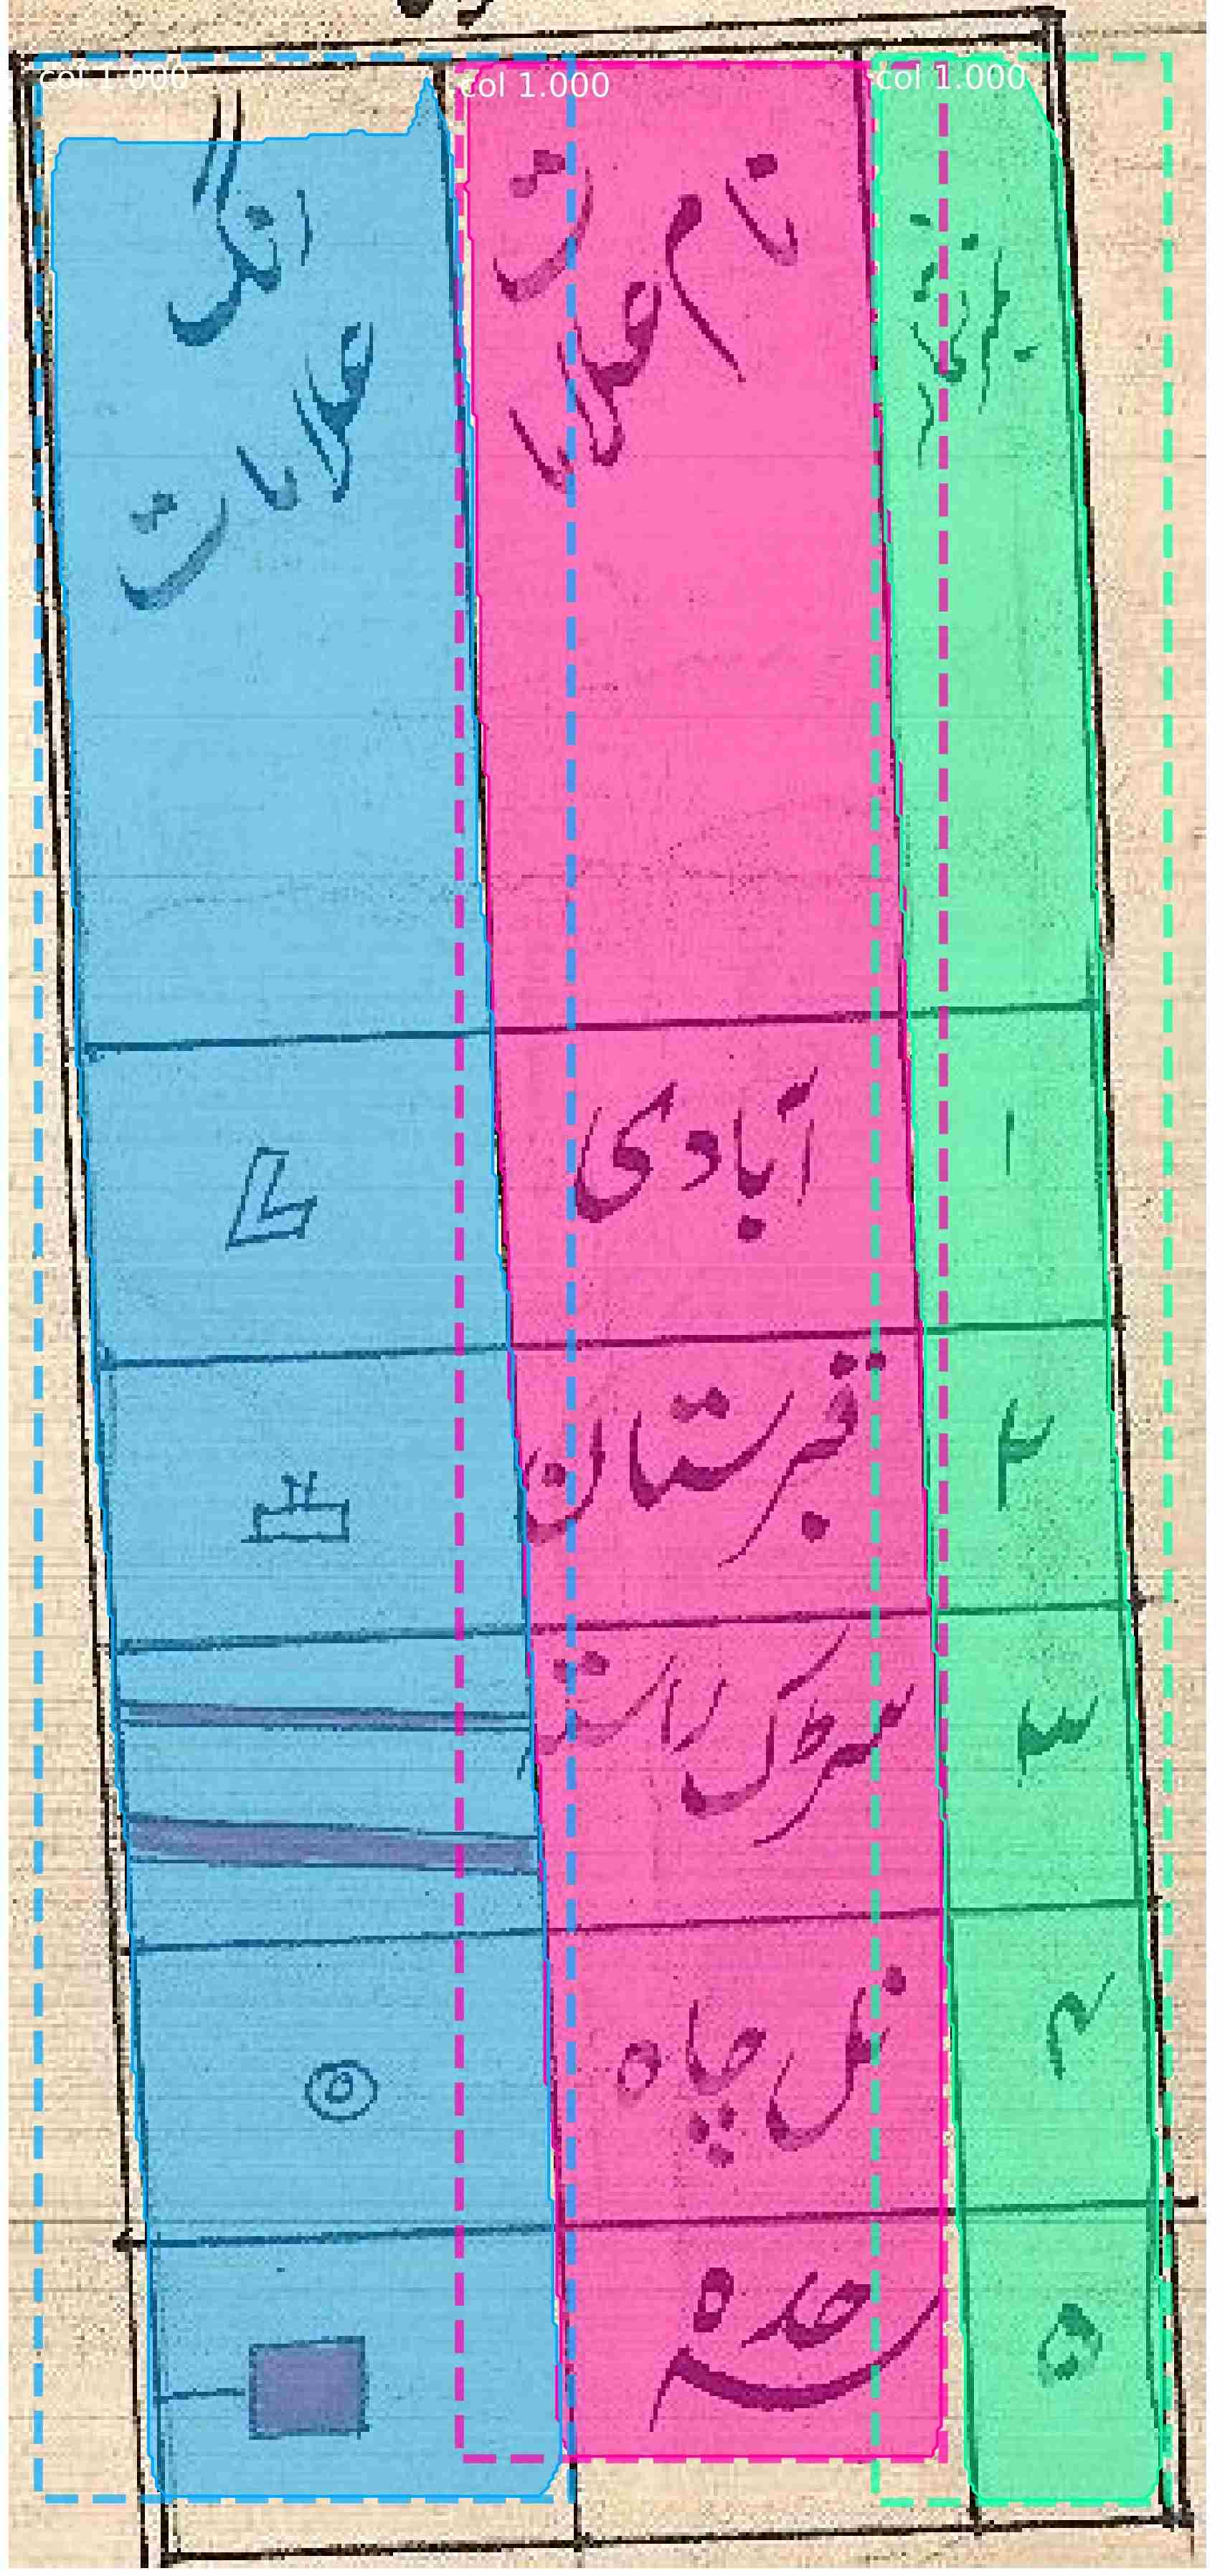
\includegraphics[width=\linewidth]{massavi_1525_0_col_mask.jpg}
    \caption{}
    \label{}
\end{subfigure}
\begin{subfigure}{0.325\linewidth}
  \centering
  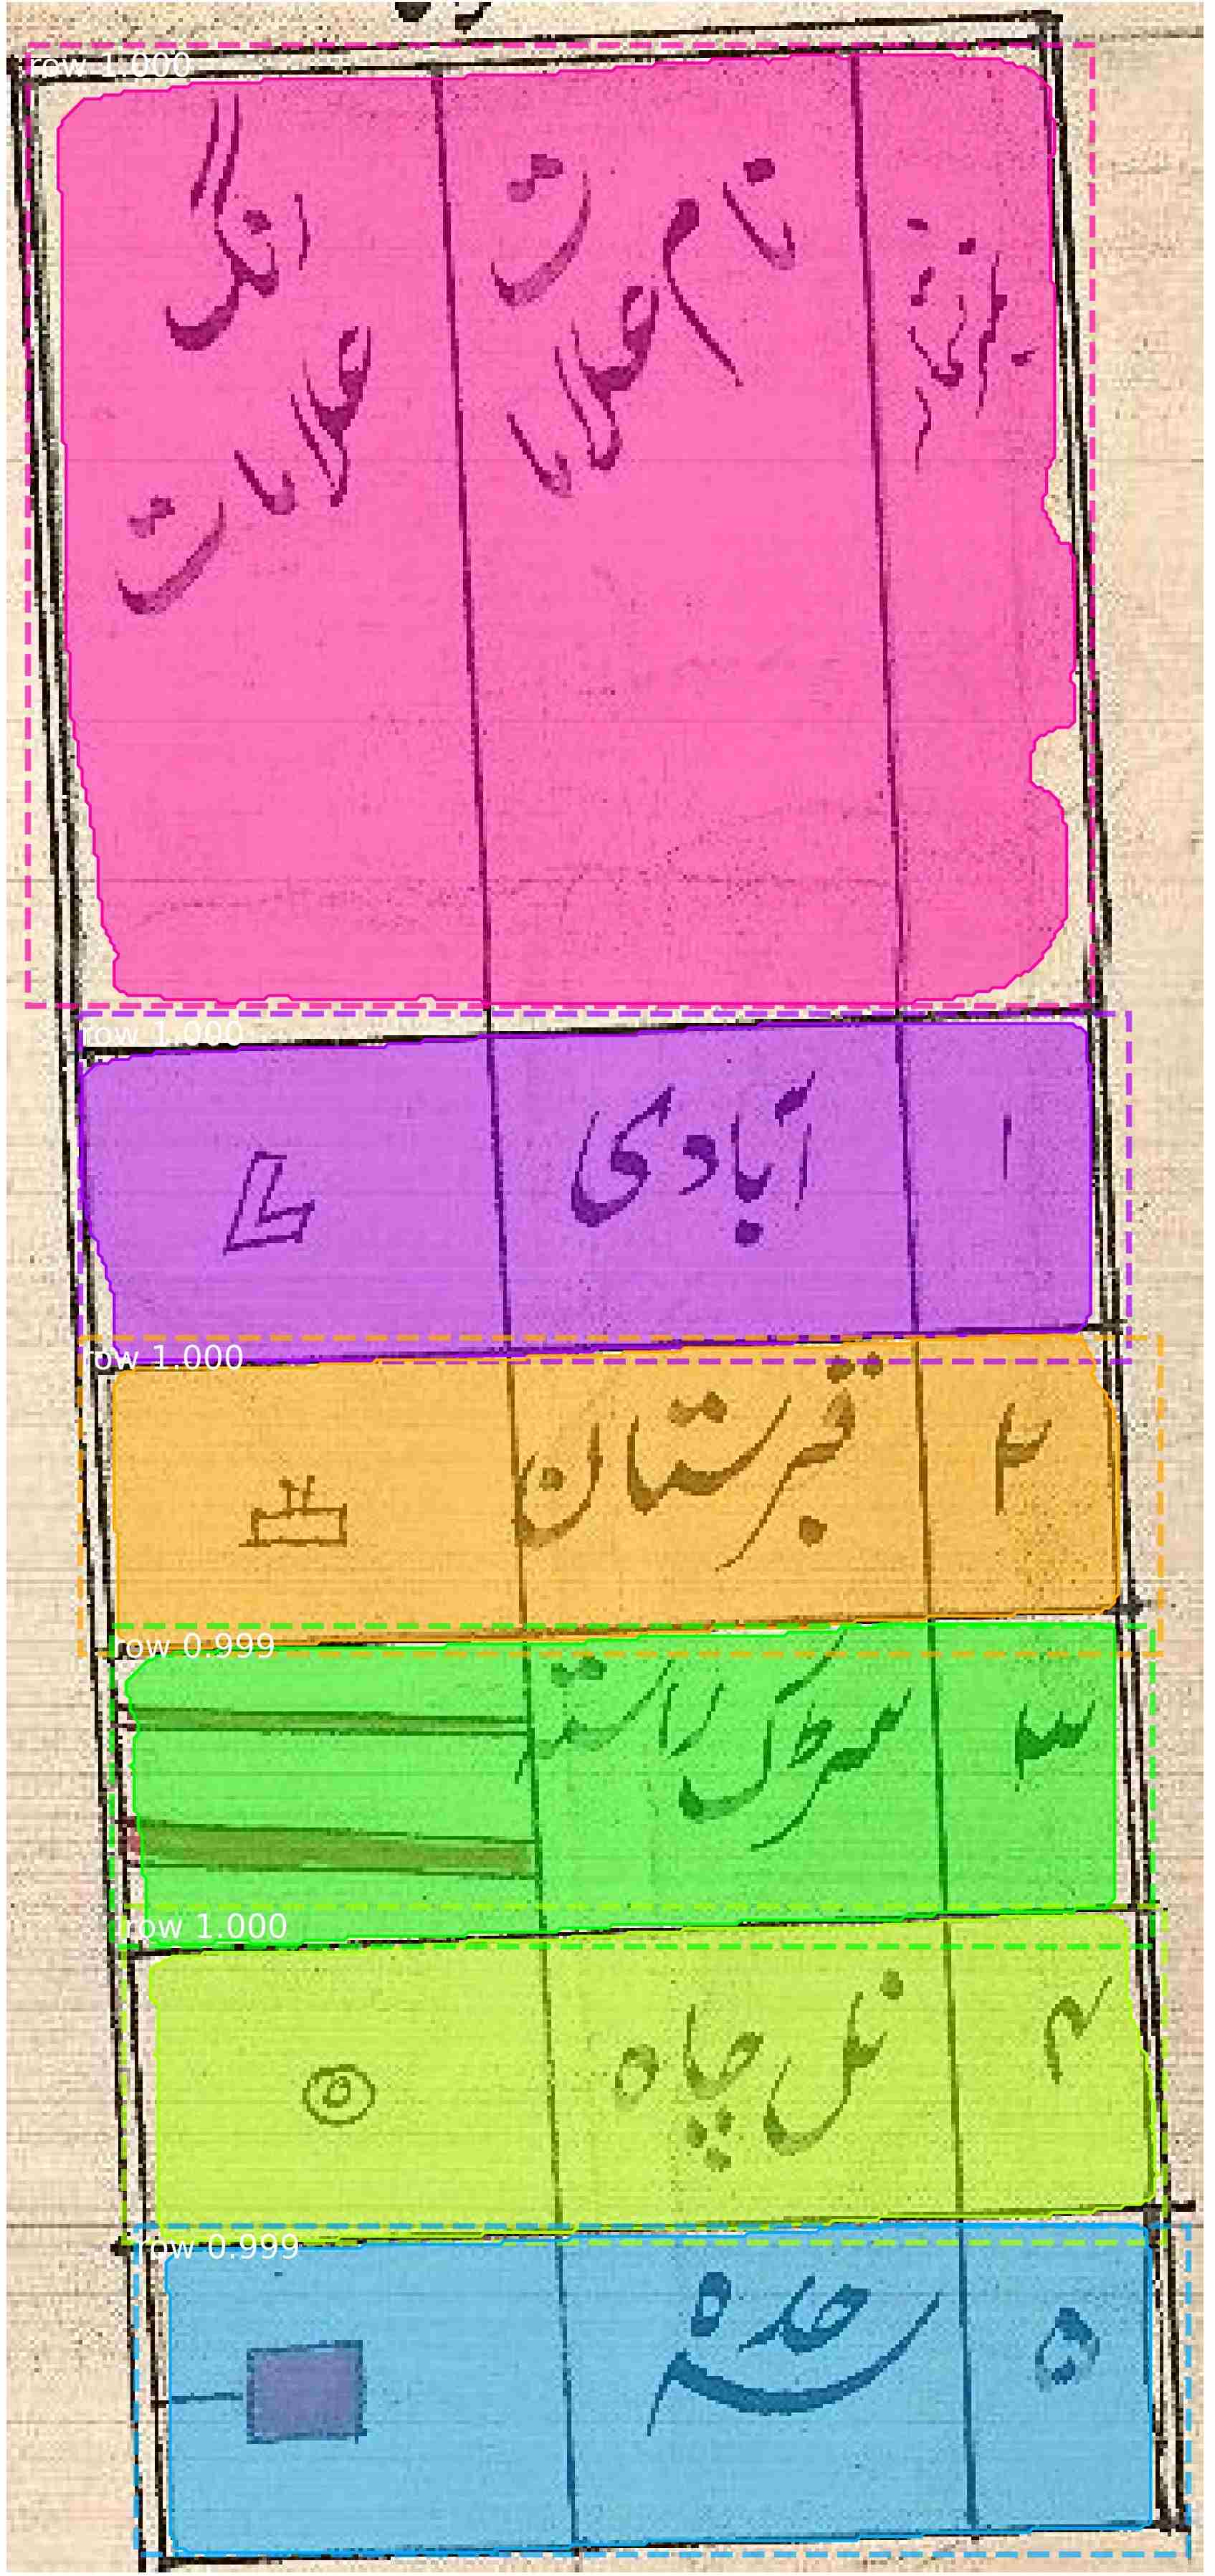
\includegraphics[width=\linewidth]{massavi_1525_rows_mask.jpg}
    \caption{}
    \label{}
\end{subfigure}
\caption{(a) is showing detection results for rows and columns which are overlapping while (b) and (c) are showing instance segmentation results for columns and rows respectively and these masks are non overlapping which helps to extract data more precisely.}
\label{fig:detVsIns}
\end{figure}
\subsection{Cell Detection}
\label{sec:expResults_cell}
After detection and structure recognition of tables we detected cells
\begin{figure*}[h!]
\centering
  % include first image
  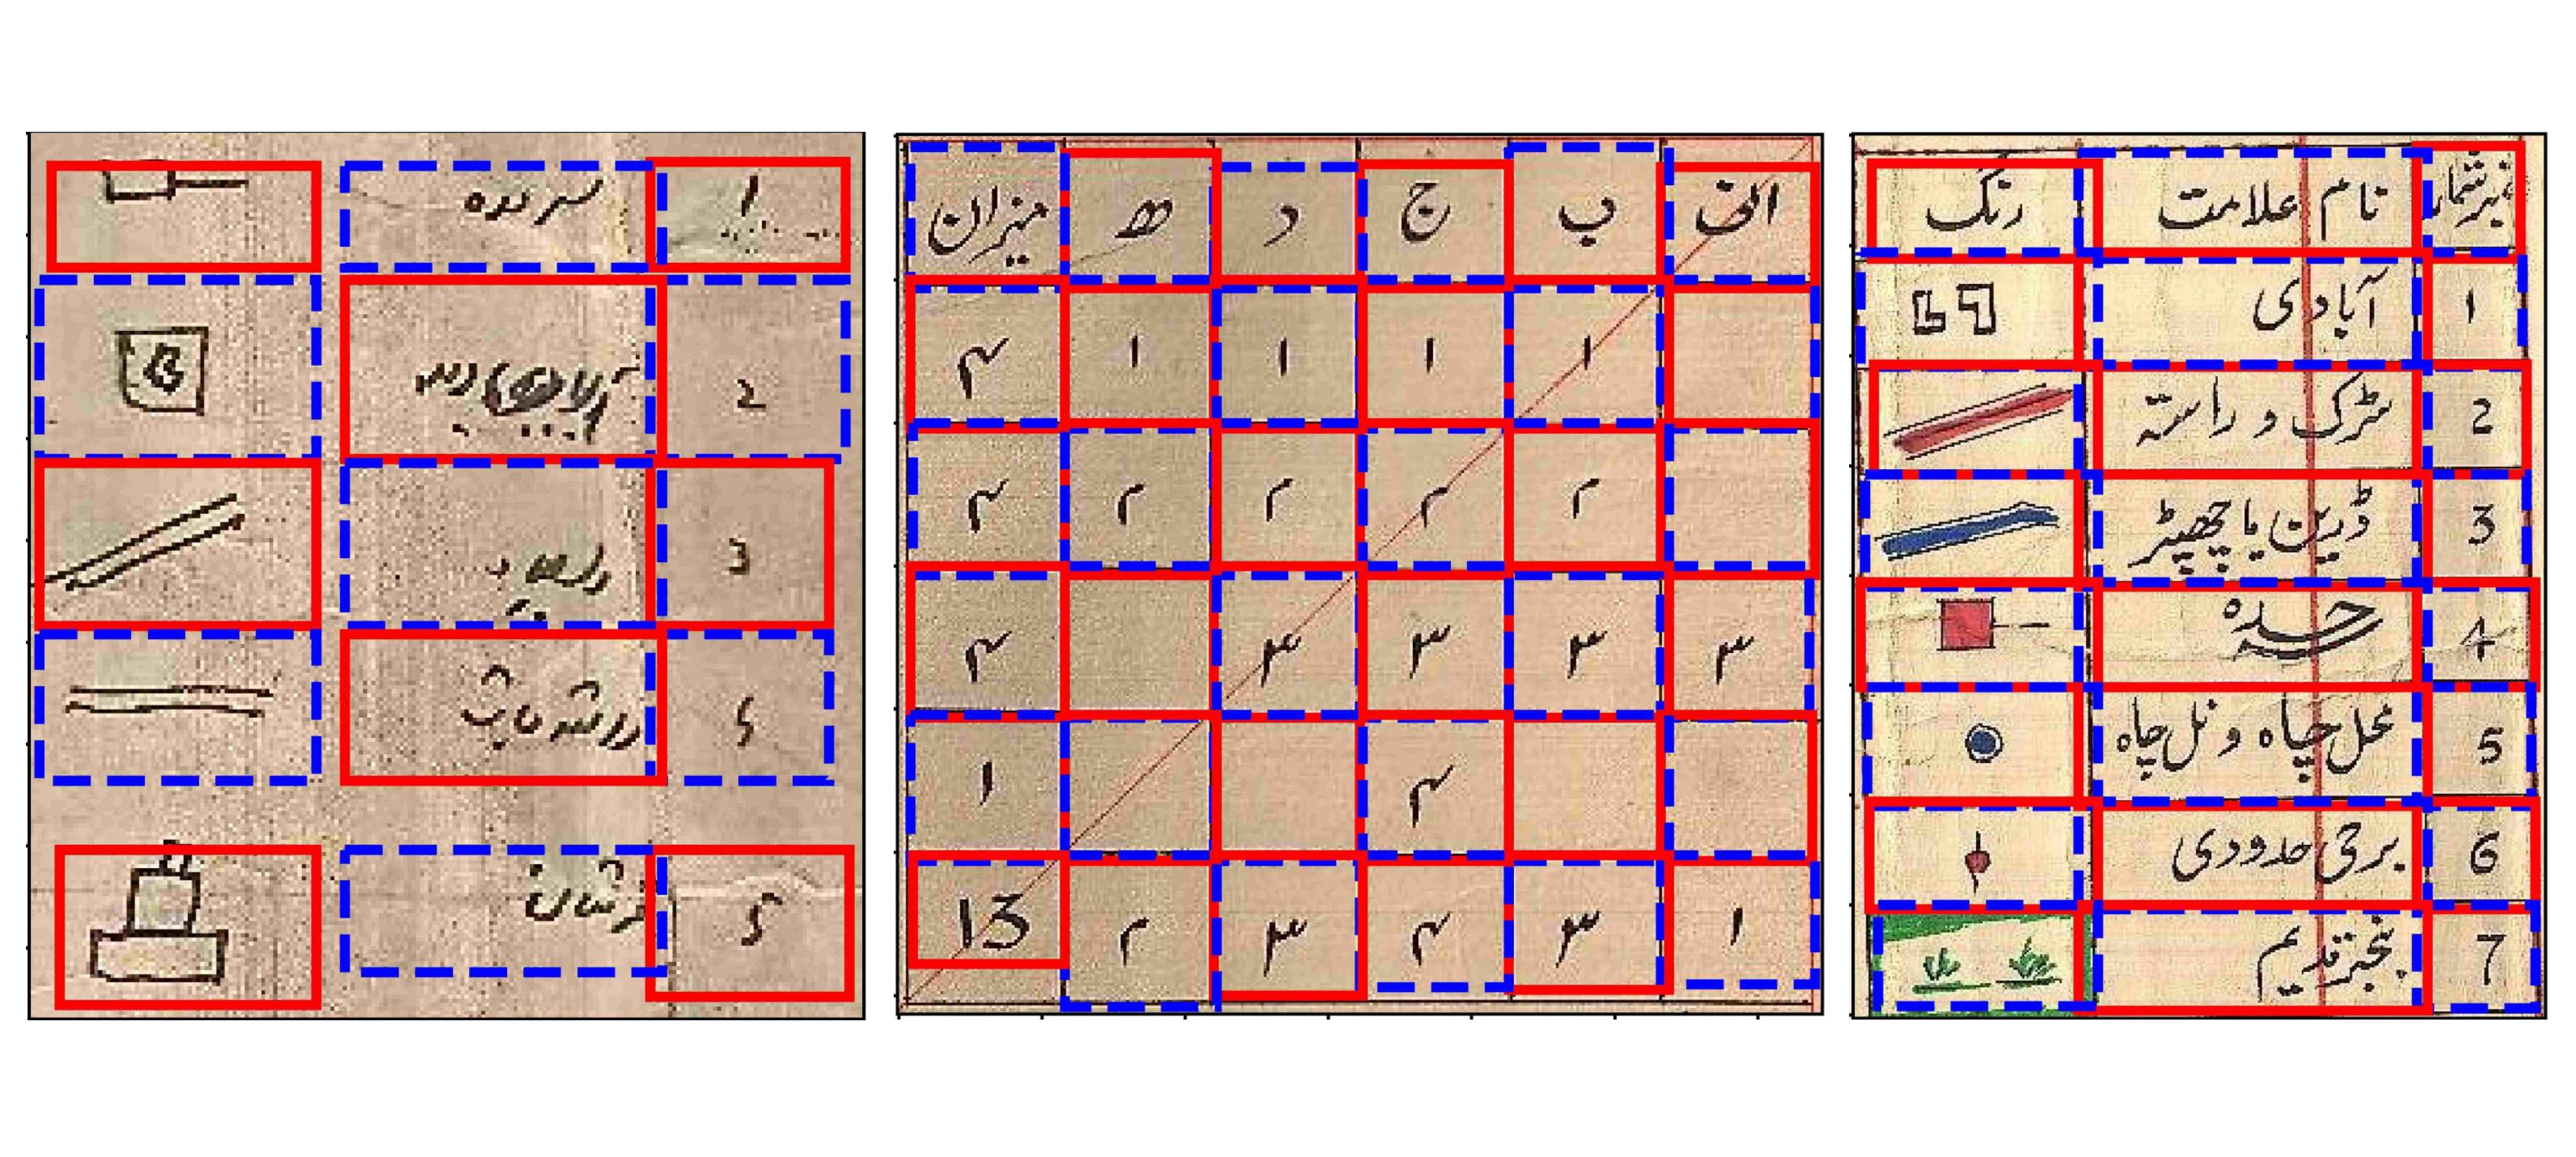
\includegraphics[width=\linewidth, keepaspectratio,angle=0]{cellDetectionResults.pdf}
    \caption{Detected cells shown in alternating red and dashed blue boxes. Left to right (border-less Legend Table, bordered Index Table, bordered Legend Table with background red grid line passing through middle column).}
    \label{fig:cellDetectionResults}
\end{figure*}
\begin{table*}[h!]
\caption{Cell Detection}
\label{tbl:cell_detection}
\centering
\resizebox{\textwidth}{!}{%
\begin{tabular}{| c | c | c |c | c | c |c | c | c |c | }
\hline
&\multicolumn{3}{|c|}{\textbf{IoU=0.5}} &\multicolumn{3}{|c|}{\textbf{IoU=0.75}}& \multicolumn{3}{|c|}{\textbf{IoU=0.9}}\\
\hline
 &\textbf{P@0.5} & \textbf{R@0.5}  & \textbf{$F_1$@0.5} & \textbf{P@0.75} & \textbf{R@0.75}  & \textbf{$F_1$@0.75}& \textbf{P@0.9} & \textbf{R@0.9}  & \textbf{$F_1$@0.9} \\ 
 \hline
 \textbf{Cells} & 92.44\% & 94.04\% & 93.24\% & 77.27\% & 78.6\% & 77.93\% & 29.16\% & 29.66\% & 29.41\% \\
 \hline
 \textbf{cells (Index Table)} & 86.08\% & 90.77\% & 88.37\% & 74.89\% & 78.97\% & 76.88\% & 31.28\% & 32.98\% & 32.11\%\\
 \hline
 \textbf{cells (Legend Table)} & 98.89\% & 98.56\% & 98.72\% & 85.28\% & 85.0\% & 85.14\% & 37.9\% & 37.78\% & 37.84\%\\
 \hline
\end{tabular}
}
\end{table*}
by the overlaps of rows and columns which are detected in the previous section. \autoref{fig:cellDetectionResults} shows cell detection results in Index and Legend Tables. \autoref{tbl:cell_detection} shows precision, recall and $F_1$ score values for cell detection in Index and Legend Tables, separate results for Index Table cells and Legend Table cells are shown in the last two rows. It can be seen that as compared to Legend Tables precision, recall and $F_1$ score values for cell detection in Index Tables are less by a significant margin which is the impact of complex structure (nested columns, row spanning cells and column spanning cells) of Index Tables. \autoref{fig:cell_graph} shows graphical representation of precision, recall and $F_1$ score values on different intersection over union threshold values.
\begin{figure}[h!]
\centering
\begin{subfigure}{0.325\linewidth}
  \centering
  % include first image
  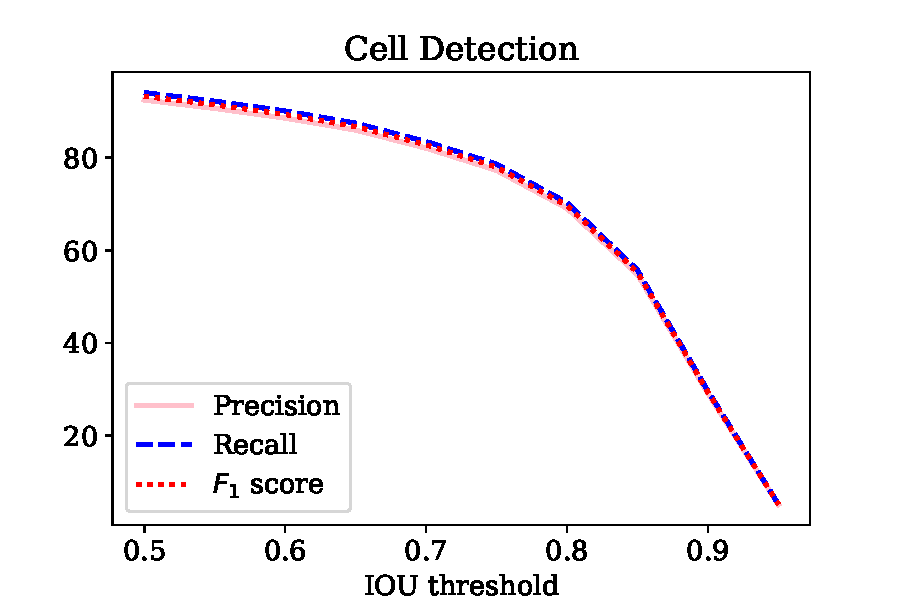
\includegraphics[width=\linewidth]{cell_pRf.pdf}
    \caption{}
    \label{}
\end{subfigure}
\begin{subfigure}{0.325\linewidth}
  \centering
  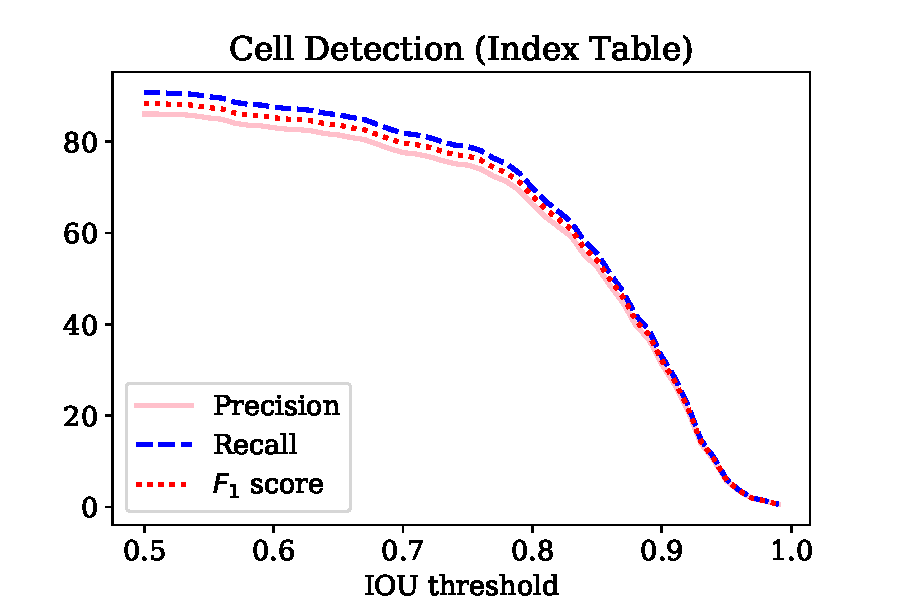
\includegraphics[width=\linewidth]{cell_index_pRf.pdf}
    \caption{}
    \label{}
\end{subfigure}
\begin{subfigure}{0.325\linewidth}
  \centering
  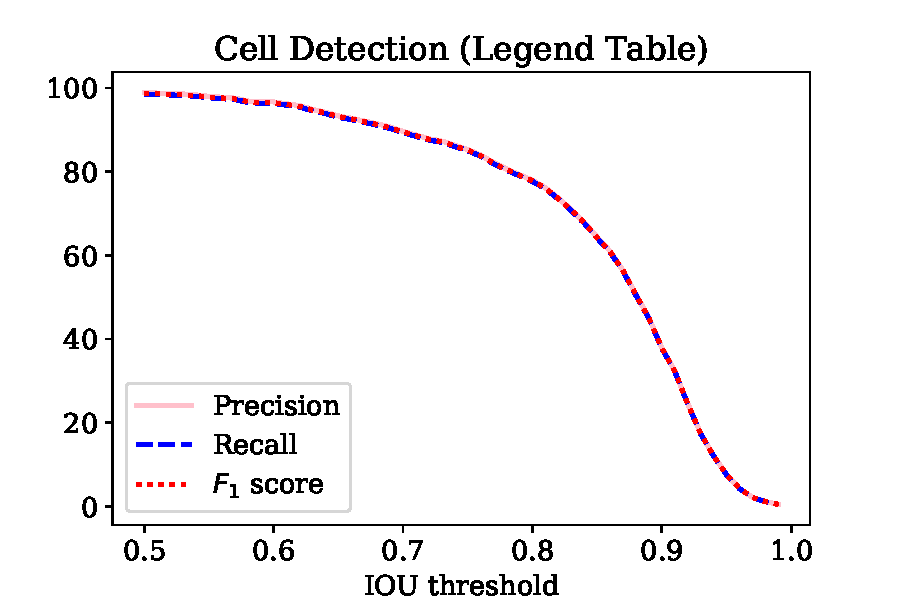
\includegraphics[width=\linewidth]{cell_legend_pRf.pdf}
    \caption{}
    \label{}
\end{subfigure}
\caption{(A) shows precision, recall and $F_1$ score curves for cell detection in both Index and Legend Tables, it can be seen that precision, recall and $F_1$ score values decrease with very small increase in IoU threshold because cells are small entities and they get affected by a slight increase in IoU threshold as compared to rows, columns and tables. (B) shows precision, recall and $F_1$ score curves for cells detection in Index Tables, difference in precision, recall and $F_1$ score values is the effect of more False Positives than False Negatives. (C) shows results for cell detection in Legend Tables having greater precision, recall and $F_1$ score values than Index Tables because Legend Tables are in regular form and more clean than Index Tables.}
\label{fig:cell_graph}
\end{figure}
\section{Conclusion}
\label{conclusion}
In this paper, we presented a deep learning based solution for detection, classification and structure recognition (row and column detection) of tables drawn in hand drawn cadastral maps. Our model can detect tables with different variations such as tables with and without horizontal and vertical lines for rows and columns even it can detect a table which has no borders. It can also detect tables with different layouts vertical tables, horizontal tables and square tables. Without reading the title of table, our model classifies table into index and legend based on the content of table and there is only one miss classification by our model on our testing dataset. After detection and classification of tables, our row and column detection model extracts rows and columns from these table for which make pixel wise predictions in order to deal with rows and columns of tables which are not orthogonal (left-skewed/right-skewed). Our model also performs very well at out of dataset images. We have also shown table detection results on non-map images which are also reasonably good. We have shown that Mask RCNN which was originally developed for object detection and instance segmentation is also very effective for detection and structure recognition of tables in historical document images. We also detect cells by the overlaps of rows and columns. We have achieved above 90\% $F_1$ score for table detection, row and column detection and cell detection. In future we will use content inside detected cells of Legend Table to spot symbols in map image and label it with the respective name of that symbol. We will extract constituent map locations using content inside detected cells of Index Table to form a village level map.
%(see Sect.~\ref{sec:1}).
%\paragraph{Paragraph headings} Use paragraph headings as needed.
%\begin{equation}
%a^2+b^2=c^2
%\end{equation}

% For one-column wide figures use
%\begin{figure}
% Use the relevant command to insert your figure file.
% For example, with the graphicx package use
  %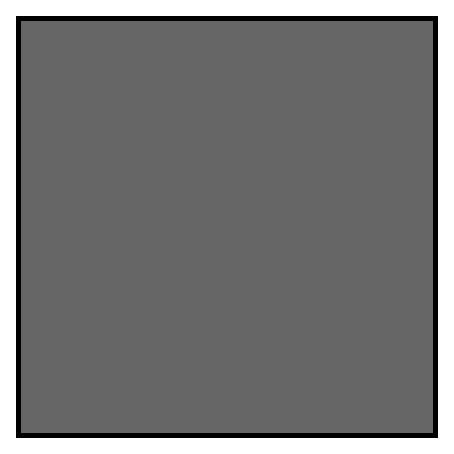
\includegraphics{example.eps}
% figure caption is below the figure
%\caption{Please write your figure caption here}
%\label{fig:1}       % Give a unique label
%\end{figure}
%
% For two-column wide figures use
%\begin{figure}
% Use the relevant command to insert your figure file.
% For example, with the graphicx package use
  %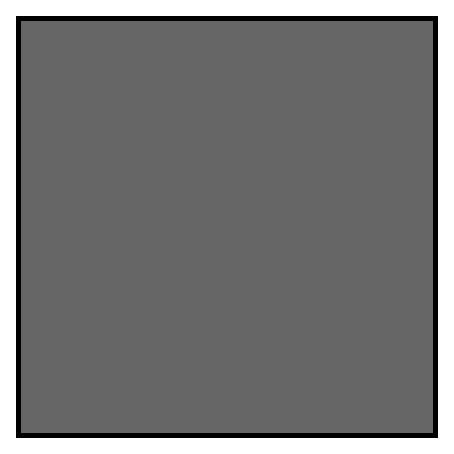
\includegraphics[width=0.75\textwidth]{example.eps}
% figure caption is below the figure
%\caption{Please write your figure caption here}
%\label{fig:2}       % Give a unique label
%\end{figure}
%
% For tables use
%\begin{table}
% table caption is above the table
%\caption{Please write your table caption here}
%\label{tab:1}       % Give a unique label
% For LaTeX tables use
%\begin{tabular}{lll}
%\hline\noalign{\smallskip}
%first & second & third  \\
%\noalign{\smallskip}\hline\noalign{\smallskip}
%number & number & number \\
%number & number & number \\
%\noalign{\smallskip}\hline
%\end{tabular}
%\end{table}


%\begin{acknowledgements}
%If you'd like to thank anyone, place your comments here
%and remove the percent signs.
%\end{acknowledgements}


% Authors must disclose all relationships or interests that 
% could have direct or potential influence or impart bias on 
% the work: 
%
% \section*{Conflict of interest}
%
% The authors declare that they have no conflict of interest.


% BibTeX users please use one of
%\bibliographystyle{spbasic}      % basic style, author-year citations
%\bibliographystyle{spmpsci}      % mathematics and physical sciences
%\bibliographystyle{spphys}       % APS-like style for physics
%\bibliography{}   % name your BibTeX data base

% Non-BibTeX users please use
\begin{thebibliography}{}
%
% and use \bibitem to create references. Consult the Instructions
% for authors for reference list style.
%
% Format for Journal Reference
\bibitem{siddiqui2018decnt}
Siddiqui, Shoaib Ahmed and Malik, Muhammad Imran and Agne, Stefan and Dengel, Andreas and Ahmed, Sheraz, Decnt: Deep deformable cnn for table detection, Journal, 6, 74151--74161 (2018)
\bibitem{schreiber2017deepdesrt}
Schreiber, Sebastian and Agne, Stefan and Wolf, Ivo and Dengel, Andreas and Ahmed, Sheraz, Deepdesrt: Deep learning for detection and structure recognition of tables in document images, IEEE, 1, 1162--1167(2017)
\bibitem{he2017multi}
He, Dafang and Cohen, Scott and Price, Brian and Kifer, Daniel and Giles, C Lee, Multi-scale multi-task fcn for semantic page segmentation and table detection, IEEE, 1, 254--261 (2017)
\bibitem{gilani2017table}
Gilani, Azka and Qasim, Shah Rukh and Malik, Imran and Shafait, Faisal, Table detection using deep learning, IEEE, 1, 771--776 (2017)
\bibitem{wang2004table}
Wang, Yalin and Phillips, Ihsin T and Haralick, Robert M, Table structure understanding and its performance evaluation, Pattern recognition, 37, 1479--1497 (2004)
\bibitem{li2019tablebank}
Li, Minghao and Cui, Lei and Huang, Shaohan and Wei, Furu and Zhou, Ming and Li, Zhoujun, Tablebank: Table benchmark for image-based table detection and recognition, arXiv preprint arXiv:1903.01949, Volume, page numbers (2019)
% Format for books
\bibitem{paliwal2019tablenet}
Paliwal, Shubham Singh and Vishwanath, D and Rahul, Rohit and Sharma, Monika and Vig, Lovekesh, 2019 International Conference on Document Analysis and Recognition (ICDAR), 128--133, IEEE, place (2019)
\bibitem{qasim2019rethinking}
Qasim, Shah Rukh and Mahmood, Hassan and Shafait, Faisal, 2019 International Conference on Document Analysis and Recognition (ICDAR), 142--147. IEEE, place (2019)
\bibitem{khan2019table}
Khan, Saqib Ali and Khalid, Syed Muhammad Daniyal and Shahzad, Muhammad Ali and Shafait, Faisal, 2019 International Conference on Document Analysis and Recognition (ICDAR), 1366--1371. IEEE, place (2019)
\bibitem{kavasidis2019saliency}
Kavasidis, Isaak and Pino, Carmelo and Palazzo, Simone and Rundo, Francesco and Giordano, Daniela and Messina, P and Spampinato, Concetto, International Conference on Image Analysis and Processing, 292--302. Springer, place (2019)
\bibitem{arif2018table}
Arif, Saman and Shafait, Faisal, 2018 Digital Image Computing: Techniques and Applications (DICTA), 1--8. IEEE, (2018)
\bibitem{shigarov2016configurable}
Shigarov, Alexey and Mikhailov, Andrey and Altaev, Andrey, Proceedings of the 2016 ACM Symposium on Document Engineering, 119--122. Publisher, place (2016)
\bibitem{kasar2015table}
Kasar, Thotreingam and Bhowmik, Tapan Kumar and Belaid, Abdel, 2015 13th International Conference on Document Analysis and Recognition (ICDAR), 1086--1090. IEEE, place (2015)
\bibitem{kasar2013learning}
Kasar, Thotreingam and Barlas, Philippine and Adam, S{\'e}bastien and Chatelain, Cl{\'e}ment and Paquet, Thierry, 2013 12th International Conference on Document Analysis and Recognition, 1185--1189. IEEE, place (2013)
\bibitem{wangt2001automatic}
Wangt, Yalin and Phillipst, IT and Haralick, Robert, Proceedings of Sixth International Conference on Document Analysis and Recognition, 528--532. IEEE, place (2001)
\bibitem{kieninger1998t}
Kieninger, Thomas and Dengel, Andreas, International Workshop on Document Analysis Systems, 255--270. Springer, place (1998)
\bibitem{ghanmi2014table}
Ghanmi, Nabil and Belaid, Abdel, 2014 14th International Conference on Frontiers in Handwriting Recognition, 146--151. IEEE, place (2014)
\bibitem{chen2012model}
Chen, Jin and Lopresti, Daniel, 2012 International Conference on Frontiers in Handwriting Recognition, 75--80. IEEE, place (2012)
\bibitem{chen2011table}
Chen, Jin and Lopresti, Daniel, 2011 International Conference on Document Analysis and Recognition, 399--403. IEEE, place (2011)
\bibitem{long2015fully}
Long, Jonathan and Shelhamer, Evan and Darrell, Trevor, Proceedings of the IEEE conference on computer vision and pattern recognition, 3431--3440. Publisher, place (2015)
\bibitem{clinchant2018comparing}
Clinchant, St{\'e}phane and D{\'e}jean, Herv{\'e} and Meunier, Jean-Luc and Lang, Eva Maria and Kleber, Florian, 2018 13th IAPR International Workshop on Document Analysis Systems (DAS), 133--138. IEEE, place (2018)
\bibitem{gupta2019table}
Gupta, Anand and Tiwari, Devendra and Khurana, Tarasha and Das, Sagorika, Smart Innovations in Communication and Computational Sciences, 361--372. Springer, place (2019)
\bibitem{prasad2020cascadetabnet}
Prasad, Devashish and Gadpal, Ayan and Kapadni, Kshitij and Visave, Manish and Sultanpure, Kavita, Proceedings of the IEEE/CVF Conference on Computer Vision and Pattern Recognition Workshops, 572--573. Publisher, place (2020)
\bibitem{girshick2014rich}
Girshick, Ross and Donahue, Jeff and Darrell, Trevor and Malik, Jitendra, Proceedings of the IEEE conference on computer vision and pattern recognition, 580--587. Publisher, place (2014)
\bibitem{girshick2015fast}
Girshick, Ross, Proceedings of the IEEE international conference on computer vision, 1440--1448. Publisher, place (2015)
\bibitem{ren2015faster}
Ren, Shaoqing and He, Kaiming and Girshick, Ross and Sun, Jian, Advances in neural information processing systems, 91--99. Publisher, place (2015)
\bibitem{redmon2016you}
Redmon, Joseph and Divvala, Santosh and Girshick, Ross and Farhadi, Ali, Proceedings of the IEEE conference on computer vision and pattern recognition, 779--788. Publisher, place (2016)
\bibitem{liu2016ssd}
Liu, Wei and Anguelov, Dragomir and Erhan, Dumitru and Szegedy, Christian and Reed, Scott and Fu, Cheng-Yang and Berg, Alexander C, European conference on computer vision, 21--37. Springer, place (2016)
\bibitem{dai2017deformable}
Dai, Jifeng and Qi, Haozhi and Xiong, Yuwen and Li, Yi and Zhang, Guodong and Hu, Han and Wei, Yichen, Proceedings of the IEEE international conference on computer vision, 764--773. Publisher, place (2017)
\bibitem{he2017mask}
He, Kaiming and Gkioxari, Georgia and Doll{\'a}r, Piotr and Girshick, Ross, Proceedings of the IEEE international conference on computer vision, 2961--2969. Publisher, place (2017)
\bibitem{zhang2018single}
Zhang, Shifeng and Wen, Longyin and Bian, Xiao and Lei, Zhen and Li, Stan Z, Proceedings of the IEEE conference on computer vision and pattern recognition, 4203--4212. Publisher, place (2018)
% etc
\end{thebibliography}
\end{document}
% end of file template.tex

